\graphicspath{{chapters/deep_learning/}}

\chapter{Deep Stochastic CCA: Bridging Multiview and Self-Supervised Learning}\label{ch:deep_learning}
\minitoc
% chktex-file 44
% chktex-file 3
\section*{Preface}

This chapter is based on work presented in \citet{chapman2023cca} and \citet{chapman2023efficient}.

\section{Introduction}

Deep CCA \citep{andrew2013deep} secured a runner-up position for the test-of-time award at ICML 2023 \citep{ICML2023TOT}.
However, its direct application has been limited in large datasets due to biased gradients in the stochastic minibatch setting.
There have since been proposals to scale-up Deep CCA in the stochastic case with adaptive whitening \citep{wang2015stochastic} and regularization \citep{chang2018scalable}, but these techniques are highly sensitive to hyperparameter tuning.

Self-Supervised Learning (SSL) methods have reached state-of-the-art in tasks such as image classification \citep{balestriero2023cookbook}, learning representations without labels that capture salient features so that they can be used for general downstream tasks.
A family of SSL methods that are closely aligned with Canonical Correlation Analysis has garnered particular interest.
This family notably includes Barlow Twins \citep{zbontar2021barlow}, VICReg \citep{bardes2021vicreg}, and W-MSE \citep{ermolov2021whitening} and they aim to transform a pair of data views into similar representations, similar to the objective of CCA. Similarly, some generative approaches to SSL\citep{sansone2022gedi} bear a striking resemblance to Probabilistic CCA\citep{bach2005probabilistic}.
These connections have started to be explored in \citet{balestriero2022contrastive}.

In this chapter, we propose a novel formulation of Deep CCA that is unbiased in the stochastic setting and scales to large datasets.
We also propose a novel SSL method, SSL-EY, that is competitive with existing methods on CIFAR-10 and CIFAR-100.
We highlight the connections between our work and existing SSL methods, and show that our method is more robust to hyperparameter tuning.

\section{Background: Deep Representation Learning}

This section explores the evolution of deep representation learning techniques, from traditional autoencoders to more sophisticated approaches like Deep Canonical Correlation Analysis (Deep CCA) and Self-Supervised Learning (SSL).

\subsection{Deep Learning and Neural Networks}
Deep learning, a subfield of machine learning, utilizes neural networks to learn complex representations from data. Neural networks are composed of interconnected layers of artificial neurons, typically including an input layer, one or more hidden layers, and an output layer. Each neuron computes a weighted sum of its inputs, followed by a nonlinear activation function.
A key component of modern neural networks is the rectified linear unit (ReLU) activation function, defined as:
\begin{equation}
\ReLU(x) = \max(0, x)
\end{equation}
ReLU and its variants have become popular due to their simplicity and effectiveness in mitigating the vanishing gradient problem during training.
The power of neural networks lies in their ability to approximate complex functions. 
The Universal Approximation Theorem \citep{cybenko1989approximation} states that a feedforward network with a single hidden layer containing a finite number of neurons can approximate any continuous function on compact subsets of $\mathbb{R}^n$, given certain mild assumptions about the activation function.
Neural networks are typically trained using backpropagation and stochastic gradient descent (SGD) or its variants. The backpropagation algorithm efficiently computes gradients of the loss function with respect to the network parameters, while SGD allows for training on large datasets by updating parameters using small batches of data.
\subsection{Autoencoders and Representation Learning}
Autoencoders represent an early approach to unsupervised representation learning. These neural networks are designed to learn compact data representations by reconstructing input data through a bottleneck layer. The basic structure of an autoencoder consists of:

An encoder function $f_{\theta}: \mathcal{X} \to \mathcal{Z}$ that maps input data to a latent representation.
A decoder function $g_{\phi}: \mathcal{Z} \to \mathcal{X}$ that attempts to reconstruct the input from the latent representation.

The autoencoder is trained to minimize a reconstruction loss:
\begin{equation}
\mathcal{L}(\theta, \phi) = \mathbb{E}_{x \sim p_{\text{data}}}[\|x - g_{\phi}(f_{\theta}(x))\|^2]
\end{equation}

Autoencoders can be viewed as a nonlinear generalization of Principal Component Analysis (PCA). In fact, a linear autoencoder with a single hidden layer and mean squared error loss is equivalent to PCA when the hidden layer dimension is less than the input dimension.
While autoencoders have been successful in various applications, they face limitations. The focus on reconstruction may lead to learning fine-grained details that are not necessarily useful for downstream tasks, and there's no explicit encouragement for the learned representations to capture meaningful features or disentangled factors of variation.

These limitations have motivated the development of more sophisticated autoencoder variants and alternative representation learning approaches.
\subsection{Variational Autoencoders}
Variational Autoencoders (VAEs) \citep{kingma2013auto} extend the autoencoder framework to learn probabilistic generative models. VAEs model the latent space as a probability distribution, typically a multivariate Gaussian, and are trained to maximize the evidence lower bound (ELBO):
\begin{equation}
\mathcal{L}_{ELBO}(\theta, \phi) = \mathbb{E}_{q_{\phi}(z|x)}[\log p_{\theta}(x|z)] - D_{KL}(q_{\phi}(z|x) || p(z))
\end{equation}
where $q_{\phi}(z|x)$ is the encoder (or inference) network, $p_{\theta}(x|z)$ is the decoder (or generative) network, and $p(z)$ is a prior distribution over the latent space.
VAEs provide a principled way to generate new samples and perform probabilistic inference, making them useful for both representation learning and generative modeling.

Research has extended Autoencoders to multiview settings, such as Multiview Autoencoders \citep{ngiam2011multimodal} which regularise autoencoders for each view to be somewhat similar to each other. Contributions of my own to this area include applications to neuroscience data \citep{lawry2023multi} and the development of a software package for multiview autoencoders \citep{florence_townend_2023_10228564}. 

However given the deep connection between Autoencoders and PCA, it is natural to consider the extension of CCA to the deep learning setting. This leads to the development of Deep CCA, which aims to learn nonlinear representations that are maximally correlated across different views.

\subsection{From Autoencoders to Deep CCA}

The objective of Deep CCA is to maximize the correlation between learned representations of different views:
\begin{align}
\label{eq:DMCCA-def}
\norm{\MCCA_K\left(Z^{(1)}, \ldots, Z^{(I)}\right)}_2
\end{align}
where $Z^{(i)} = f^{(i)}(X^{(i)}; \theta^{(i)})$ are the learned representations for each view.
\begin{figure}
\centering
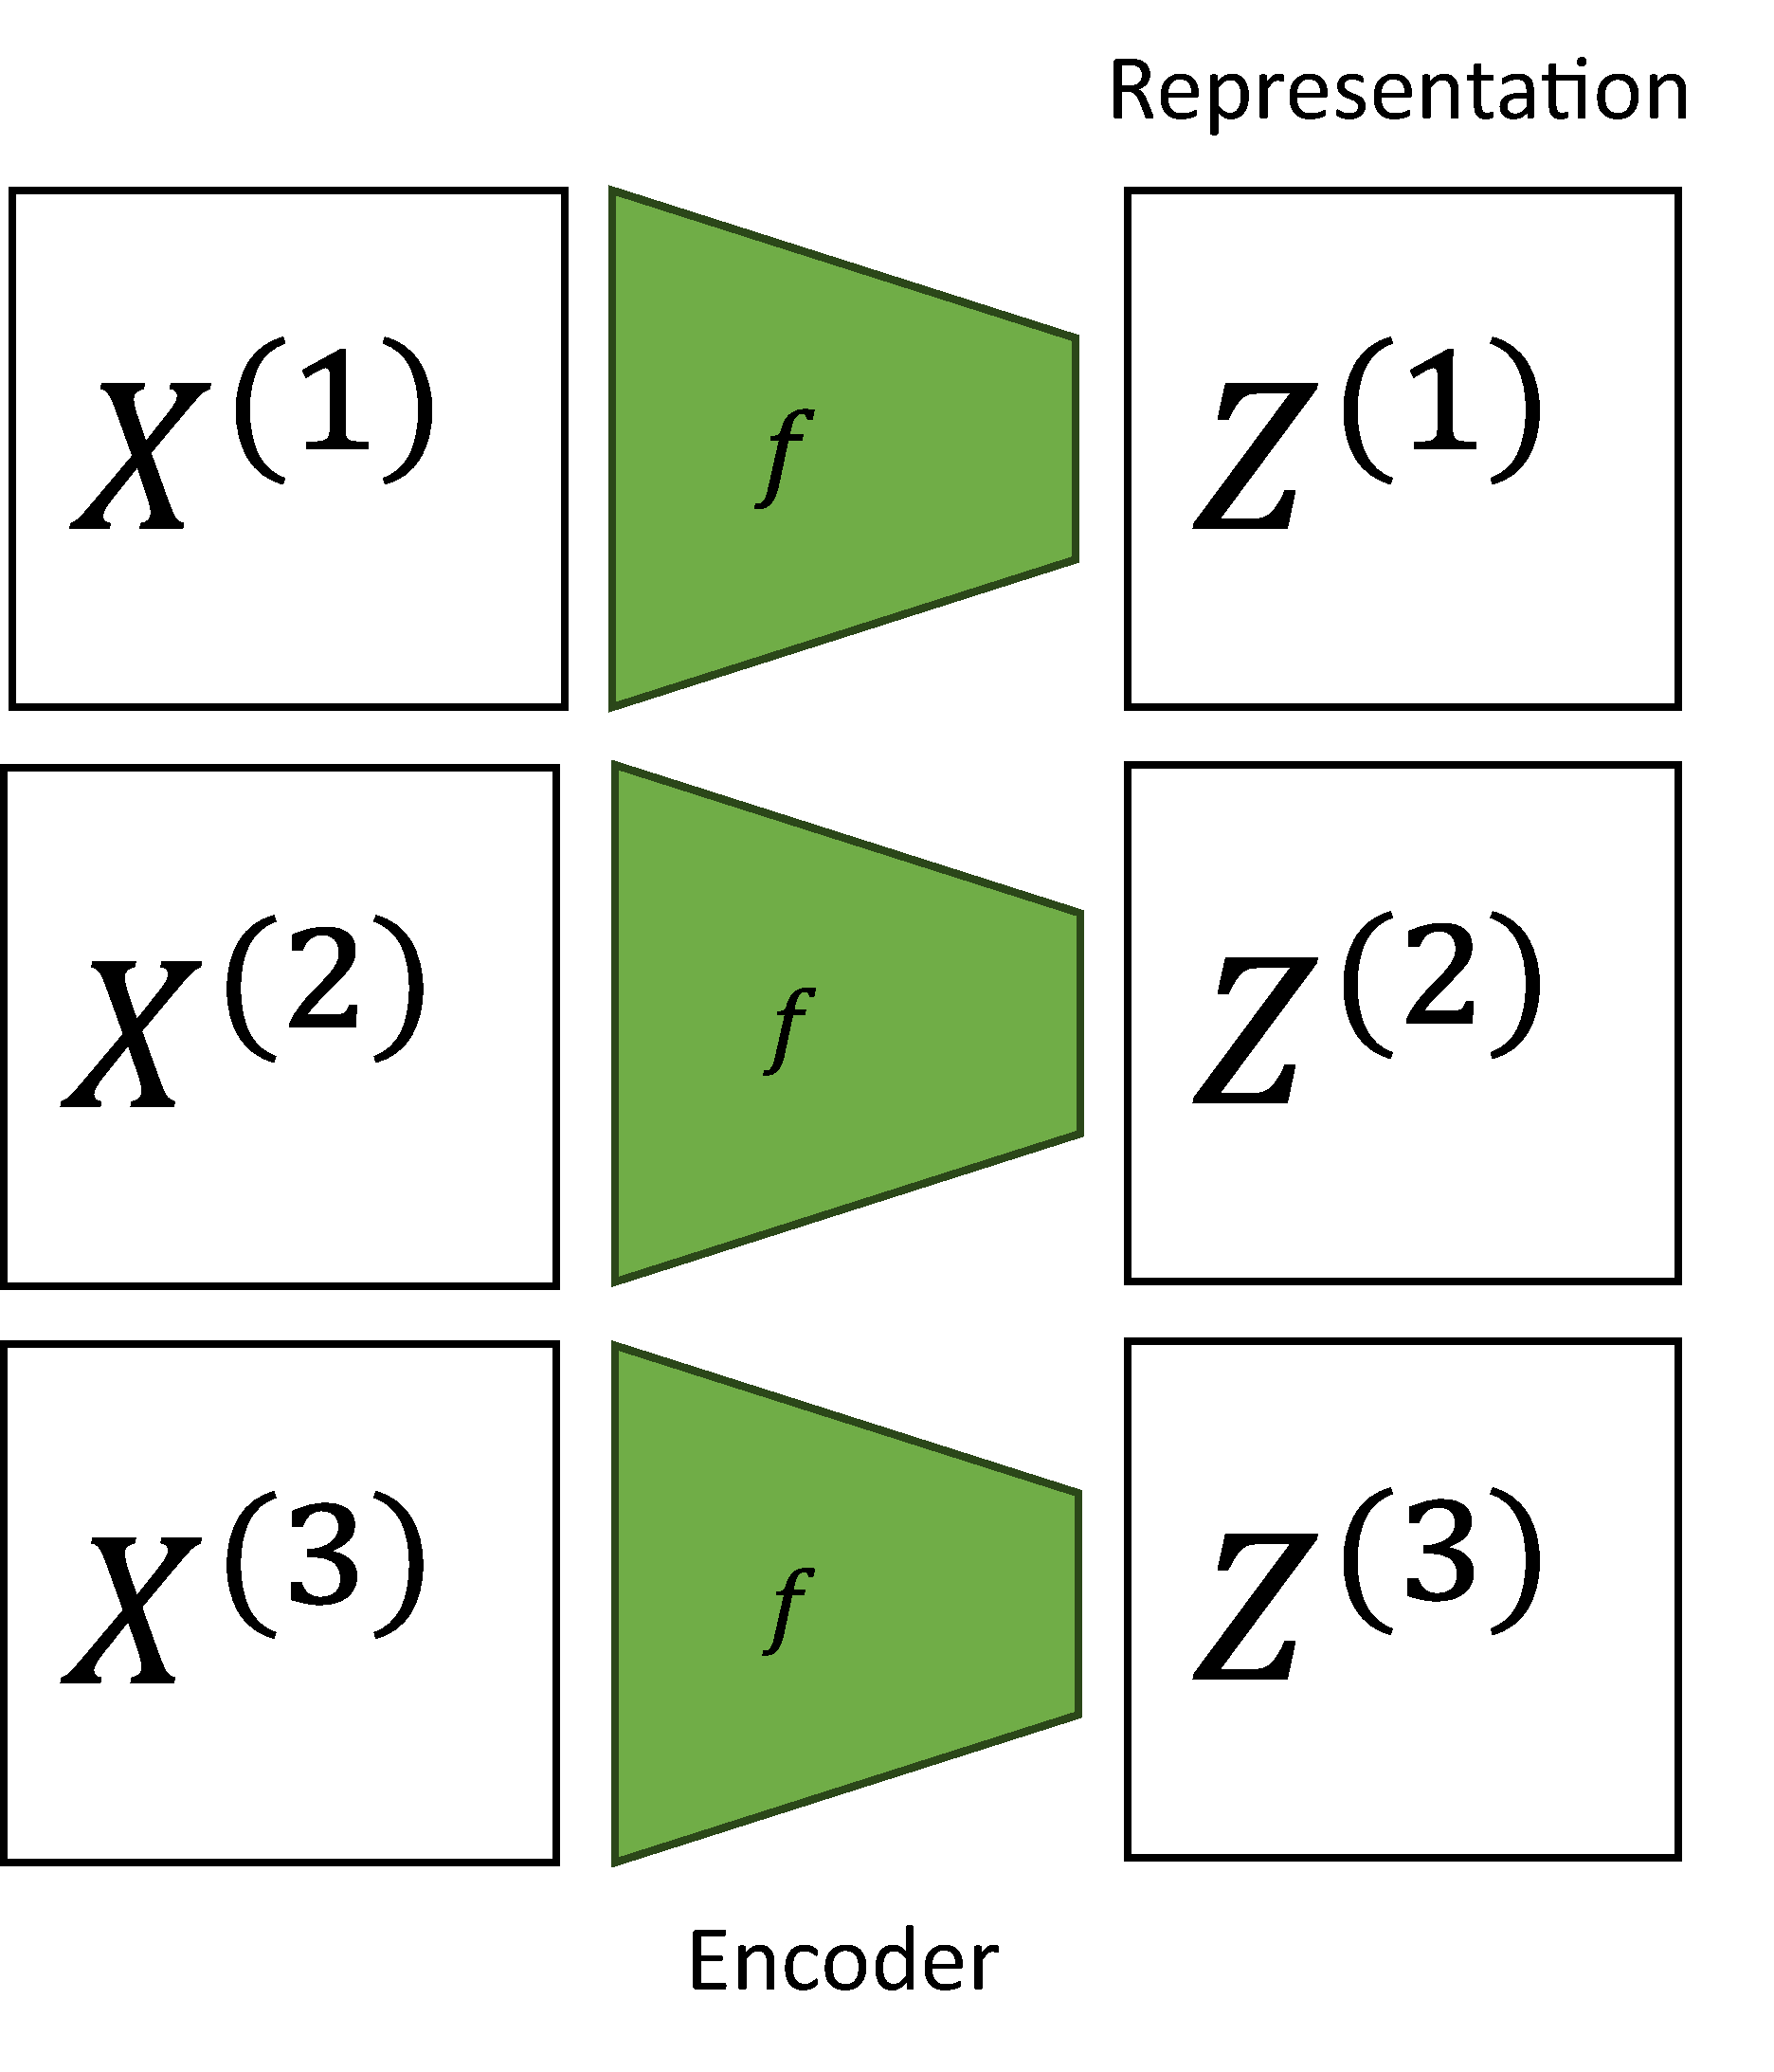
\includegraphics[width=0.5\textwidth]{figures/dcca_schematic}
\caption{Schematic of the Deep CCA approach highlighting the nonlinear transformation of data into correlated views.}
\label{fig:dcca_schematic}
\end{figure}
Figure \ref{fig:dcca_schematic} illustrates how Deep CCA transforms data from different views through neural networks to achieve correlated representations. This approach allows for capturing complex, nonlinear relationships between views that linear methods might miss.

\subsubsection{Full-batch Deep CCA}
The full-batch approach of Deep CCA, formulated by \citet{andrew2013deep}, maximizes correlation using the following loss function:

\begin{align}\label{eq:T_definition}
    T          & = \left(\text{cov}(Z^{(1)})\right)^{-\frac{1}{2}} Z^{(1)\top} Z^{(2)} \left(\text{cov}(Z^{(2)})\right)^{-\frac{1}{2}} \\
    \LRayleigh & = -\Tr(T)
\end{align}

We refer to this as the Rayleigh loss because it effectively maximizes the Generalized Rayleigh Quotient associated with the canonical correlation problem. While theoretically sound, this approach faces significant scalability issues with large datasets.

The Rayleigh loss is only valid for full batch gradient descent, which becomes computationally infeasible for large datasets. This limitation has led to numerous issues reported on the GitHub implementation, with users experiencing problems with ill-conditioned matrices and exploding gradients. These problems arise because the covariance matrices can become singular or nearly singular when working with small batches or high-dimensional data, leading to instability in the matrix inversions required by the loss function.

\subsubsection{DCCA-STOL}
DCCA-STOL, proposed by \citet{wang2015unsupervised}, attempts to use the full-batch objective with large mini-batches but suffers from biased gradients due to the matrix inversions in Equation \eqref{eq:T_definition}. This bias is fundamentally a consequence of Jensen's inequality applied to the inverse of a random variable. 

For a positive random variable $X$, Jensen's inequality states that:

\begin{equation}
\frac{1}{E[X]} \leq E[\frac{1}{X}]
\end{equation}

This inequality arises because $f(x) = \frac{1}{x}$ is a convex function for $x > 0$. 

To illustrate this, consider a simple example: Let $X$ be a random variable that is 1 with probability 0.5 and 0.1 with probability 0.5. Then:

\begin{align}
    E[X] &= 0.5 \cdot 1 + 0.5 \cdot 0.1 = 0.55 \\
    \frac{1}{E[X]} &= \frac{1}{0.55} \approx 1.82 \\
    E[\frac{1}{X}] &= 0.5 \cdot \frac{1}{1} + 0.5 \cdot \frac{1}{0.1} = 0.5 + 5 = 5.5
\end{align}

As we can see, $\frac{1}{E[X]} < E[\frac{1}{X}]$, confirming the inequality. 

In the context of DCCA-STOL, this inequality leads to biased estimates when inverting covariance matrices estimated from mini-batches. The expectation of the inverse of the sample covariance matrix is not equal to the inverse of the expected covariance matrix. This bias necessitates batch sizes larger than the representation size, limiting the method's practical application.

The problem becomes even more severe when the batch size is smaller than the representation dimension. In this case, the sample covariance matrix is guaranteed to be singular. To understand why, consider that a batch of size $n$ in a $d$-dimensional space (where $n < d$) can only span an $n$-dimensional subspace. Consequently, the sample covariance matrix will have at most rank $n$, making it singular in the $d$-dimensional space.

For singular matrices, the inverse is undefined, which is equivalent to division by zero in the scalar case. This causes Jensen's inequality to blow up to infinity, making the optimization problem ill-posed and impossible to solve.

Even when the batch size is slightly larger than the representation dimension, the covariance matrix can be nearly singular, leading to numerical instability and unreliable results.

A practical example illustrates the severity of this issue: Consider training deep neural networks on 3D MRI scans. Due to memory constraints of GPUs, it's often impossible to use large batch sizes for such high-dimensional data. If we attempt to use small batch sizes with the Rayleigh or STOL objective, we encounter singular (when batch size < representation dimension) or near-singular (when batch size $\approx$ representation dimension) matrices. The singularity effectively causes division by zero in Jensen's inequality, blowing up the expectation to infinity.

This problem has caused confusion for many GitHub users (including myself!) who attempted to implement these methods. The nuanced nature of this issue is not immediately apparent, leading to unexpected behavior and optimization failures. It's crucial to understand that to even get the optimization to run, we require batch sizes substantially larger than the representation dimension, before even considering problems of bias. This requirement severely limits the applicability of the method to high-dimensional data or large models, as it demands enormous batch sizes that often exceed available computational resources.

\subsubsection{Deep MCCA and Deep GCCA}
Extensions such as Deep MCCA \citep{somandepalli2019multimodal} and Deep GCCA \citep{benton2017deep} are multiview extensions of Deep CCA. 
Recalling the notation from \ref{sec:dim-reduction}, where $\hat{C}(\theta)$ and $\hat{V}(\theta)$ are the mini-batch estimates of the between-view and within-view covariance matrices, respectively, the loss function for Deep MCCA is given by:

\begin{align}
    T      & = \left(\hat{V}(\theta)^{-\frac{1}{2}} \hat{C}(\theta)\hat{V}(\theta)^{-\frac{1}{2}}\right) \\
    \LDMCCA & = -\Tr(T)
\end{align}

However, these methods still require large batch sizes due to biased gradients from small mini-batch covariance matrices. This issue stems from the same problem as DCCA-STOL: the matrix inversions in the loss function lead to biased estimates when using small mini-batches, again due to Jensen's inequality.

\subsubsection{Adaptive Whitening Methods}
Adaptive whitening methods \citep{wang2015stochastic, chang2018scalable} offer another solution to the scalability problem. These methods aim to approximate the matrix inversion in the loss function without actually inverting the matrix, functioning similarly to a preconditioner in optimization. By doing so, they attempt to mitigate the bias introduced by direct matrix inversion on small mini-batches.

One such method is DCCA-NOI \citep{wang2015unsupervised}, which uses Nonlinear Orthogonal Iteration to approximate the whitening transformation. The loss function of DCCA-NOI is:

\begin{align}
    \LNOI & = |{\tilde{\Sigma}_{11}}^{-\frac{1}{2}} Z\sps{1}-{\tilde{\Sigma}_{22}}^{-\frac{1}{2}} Z\sps{2}|^2_F
\end{align}

where $\tilde{\Sigma}_{11}$ and $\tilde{\Sigma}_{22}$ are estimates of the covariance matrices of $Z\sps{1}$ and $Z\sps{2}$. The adaptive whitening approach aims to iteratively refine these estimates over time, potentially allowing for smaller batch sizes. However, these methods introduce a time constant that complicates analysis and requires extensive tuning. This time constant represents the rate at which the whitening estimates are updated, and finding the right balance between stability and adaptivity can be challenging.

\subsection{Self-Supervised Learning and Joint Embedding}

Self-Supervised Learning (SSL) has emerged as a powerful approach for learning representations from unlabeled data. A key strategy in SSL involves creating joint embeddings of augmented data, typically images.

\begin{figure}
\centering
\tikz{
    \node[latent, align=center] (x) {Original Data\\$X$};
    \node[obs, below left=of x, align=center] (x1) {Augmented Data\\$X^{(1)}$};
    \node[obs, below right=of x, align=center] (x2) {Augmented Data\\$X^{(2)}$};
    \edge{x} {x1}
    \edge{x} {x2}
}
\caption{Joint Embedding Data Generation Process in SSL}
\label{fig:joint_embedding}
\end{figure}

SSL methods often employ an encoder-projector model:

\begin{figure}
\centering
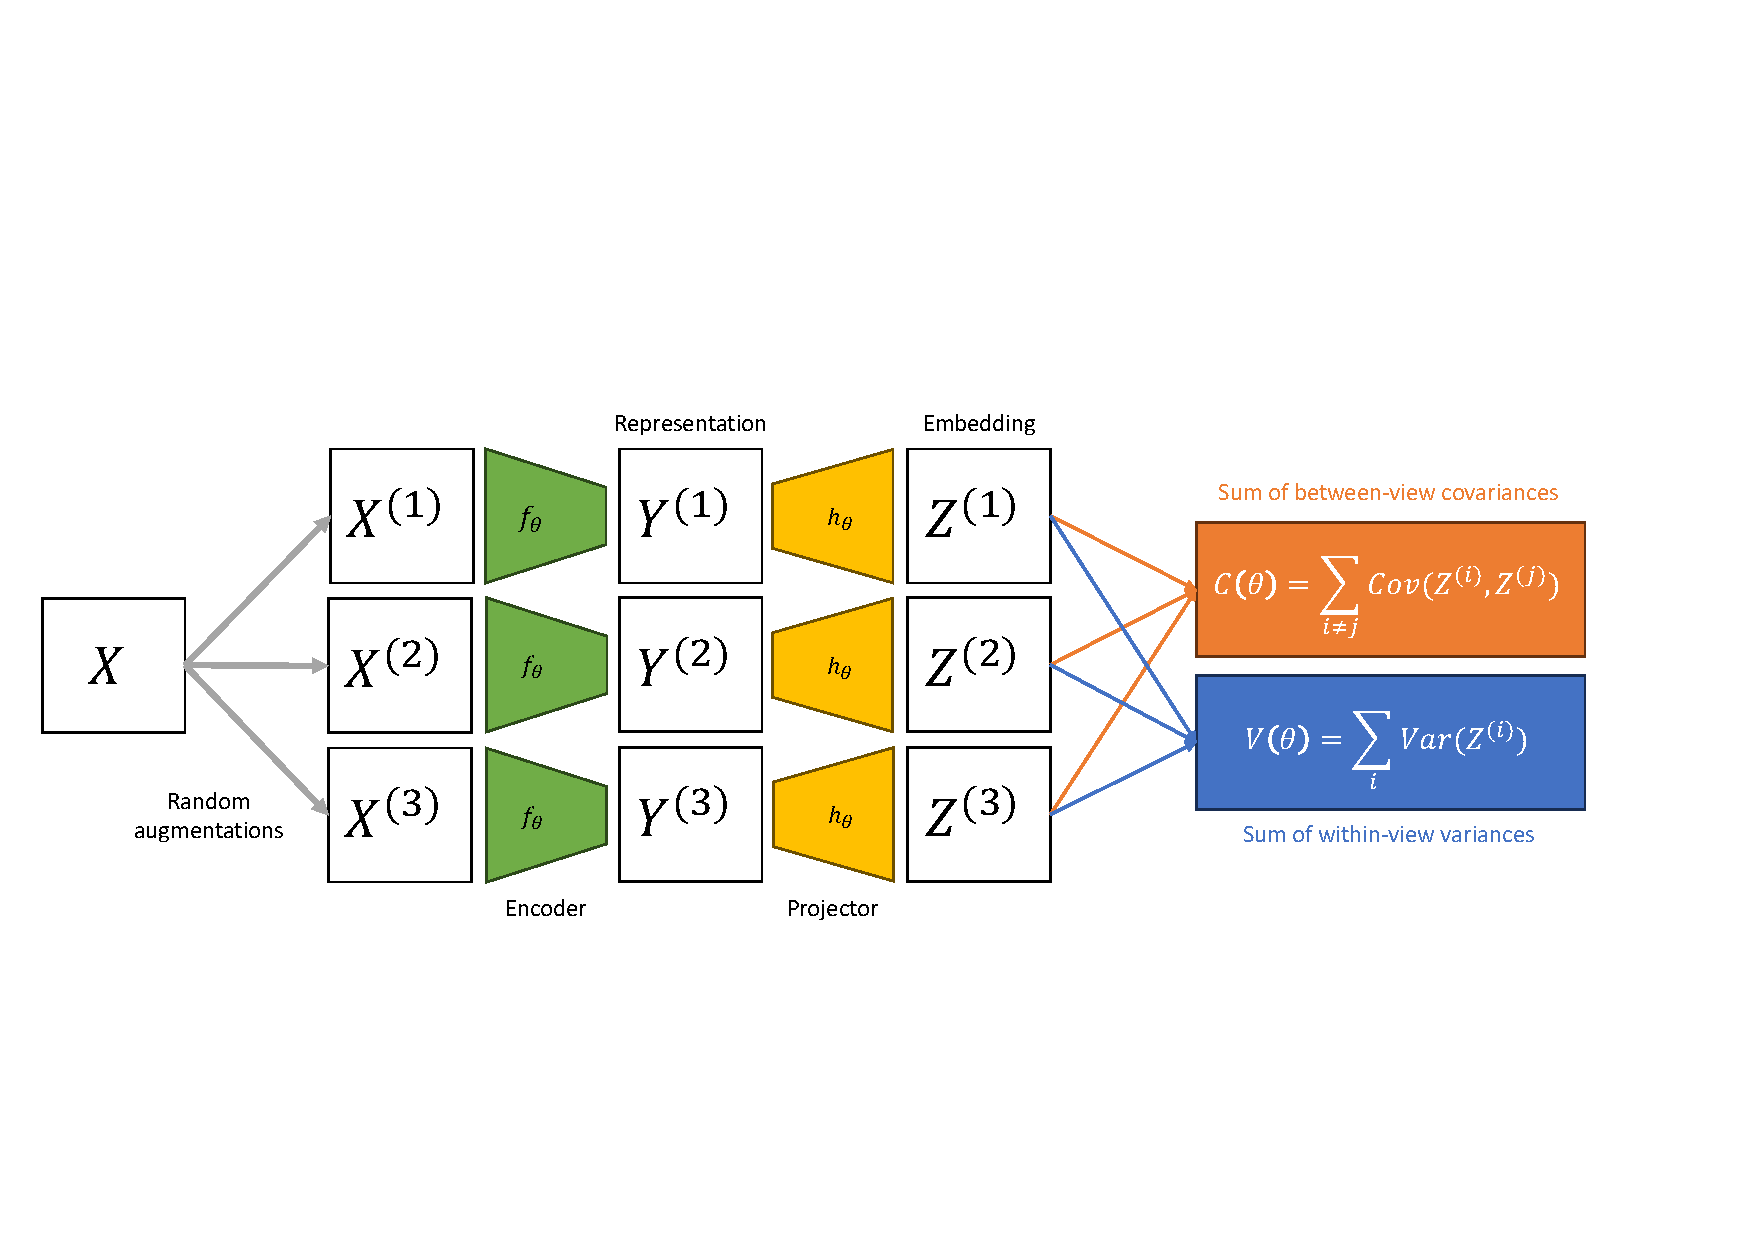
\includegraphics[width=0.9\textwidth]{figures/ssl_schematic}
\caption{Encoder-Projector Model in SSL}
\label{fig:sslschematic}
\end{figure}

\subsubsection{CCA-based SSL Methods: Barlow Twins and VICReg}

Two prominent self-supervised learning (SSL) methods, Barlow Twins and VICReg (Variance-Invariance-Covariance Regularization), utilize objectives that share similarities with Canonical Correlation Analysis principles. These methods aim to learn representations that are invariant to data augmentations while maintaining informative and decorrelated features.

\paragraph{Barlow Twins}
Introduced by \citet{zbontar2021barlow}, Barlow Twins is inspired by the redundancy reduction principle in neuroscience \citep{barlow1961possible}. The method aims to create embeddings that are invariant to distortions of the input sample while avoiding the collapse of the learned representations.

\textbf{Barlow Twins Loss:}
\begin{equation}
\LBT = \underbrace{\gamma \mathbb{E} \norm{Z^{(1)} - Z^{(2)}}^2}_{\text{Invariance}} + \underbrace{\beta \sum_{\substack{k,l=1 \\ k \neq l}}^K \Cov(\hat{Z}^{(i)}_k, \hat{Z}^{(i)}_l)^2}_{\text{Redundancy Reduction}}
\end{equation}

The loss function consists of two terms:
\begin{itemize}
    \item \textbf{Invariance term:} Encourages the embeddings of distorted versions of a sample to be similar.
    \item \textbf{Redundancy reduction term:} Minimizes the redundancy between the dimensions of the embedding vectors.
\end{itemize}

\paragraph{VICReg}
VICReg, proposed by \citet{bardes2021vicreg}, builds upon the ideas of Barlow Twins but introduces an additional variance term to explicitly encourage the embeddings to be diverse and avoid dimensional collapse.

\textbf{VICReg Loss:}
\begin{equation}
\begin{split}
\LVR = &\underbrace{\gamma \mathbb{E} \norm{Z^{(1)} - Z^{(2)}}^2}_{\text{Invariance}} + \\
&\underbrace{\sum_{i \in \{1,2\}} \alpha \sum_{k=1}^K \left(1 - \sqrt{\Var(Z^{(i)}_k)}\right)_+}_{\text{Variance}} + 
\underbrace{\beta \sum_{\substack{k,l=1 \\ k \neq l}}^K \Cov(Z^{(i)}_k, Z^{(i)}_l)^2}_{\text{Covariance}}
\end{split}
\end{equation}

The VICReg loss function comprises three terms:
\begin{itemize}
    \item \textbf{Invariance term:} Similar to Barlow Twins, it encourages the embeddings of augmented versions of a sample to be close.
    \item \textbf{Variance term:} Ensures that the variance of each embedding dimension is above a certain threshold, preventing dimensional collapse.
    \item \textbf{Covariance term:} Minimizes the covariance between different dimensions of the embeddings, promoting decorrelation.
\end{itemize}

\paragraph{Relation to CCA}
Both Barlow Twins and VICReg share similarities with CCA in their objectives:

\begin{itemize}
    \item The invariance terms in both methods are analogous to maximizing correlation in CCA, as they encourage similar representations for related inputs.
    \item The redundancy reduction term in Barlow Twins and the covariance term in VICReg are similar to the orthogonality constraints in CCA, promoting decorrelated features.
    \item VICReg's variance term can be seen as a way to ensure that the learned representations capture meaningful variations in the data, which is implicitly achieved in CCA through its formulation.
\end{itemize}

These methods demonstrate the effectiveness of CCA-inspired principles in self-supervised learning, providing a promising direction for learning robust and informative representations without relying on labeled data.

\section{Methods: DCCA-EY and SSL-EY, extending GEP-EY to Deep Learning}

Building upon the Eckart-Young inspired objective introduced in the previous chapter, we now extend our approach to non-linear transformations of the data. The key idea is to replace linear representations with non-linear ones, effectively optimizing the representation of the original data to maximize canonical correlations.

Recall the objective function from the previous chapter:
\begin{align}
\LEY(\theta) = -2 \Tr C(\theta) + \norm{V_\alpha(\theta)}_F^2
\end{align}
In this chapter, we consider non-linear transformations of the data, defined as:
\begin{align}
Z^{(i)} = f^{(i)}(X^{(i)}; \theta^{(i)})
\end{align}
where $f^{(i)}$ are non-linear functions (typically neural networks) parameterized by $\theta^{(i)}$.

\subsection{Deep Multiview Canonical Correlation Analysis (DCCA-EY)}

We first show that our objective recovers Deep Multi-view CCA at any local optimum, assuming a final linear layer in each neural network.

\begin{restatable}{lemma}{recoverDeepCCA}[Objective recovers Deep Multi-view CCA]\label{lem:recover-DeepCCA}
    Assume that there is a final linear layer in each neural network $f\sps{i}$.
    Then at any local optimum, $\hat{\theta}$, of the population problem, we have
    \begin{align*}
        \LEY(\hat{\theta}) = - \norm{\MCCA_K(\hat{Z})}_2^2
    \end{align*}
    where $\hat{Z} = f_{\hat{\theta}}(X)$.
    Therefore, $\hat{\theta}$ is also a local optimum of objectives from \citet{andrew2013deep, somandepalli2019multimodal} as defined in \cref{eq:DMCCA-def}.
\end{restatable}

\begin{proof}[Proof sketch:]
    Consider treating the penultimate-layer representations as fixed, and optimising over the weights in the final layer.
    This is precisely equivalent to optimising the Eckhart-Young loss for linear CCA where the input variables are the penultimate-layer representations.
    So by \cref{prop:EY-charac} the optimal value is the negative sum of squared generalised eigenvalues.
\end{proof}

This result shows that our objective, which we call \textbf{DCCA-EY}, is a valid generalization of Deep CCA and can be used to learn correlated non-linear representations.

\subsection{Application to Self-Supervised Learning (SSL-EY)}

We can directly apply the DCCA-EY approach to the self-supervised learning (SSL) setting, which we call \textbf{SSL-EY}. The key differences between DCCA-EY and SSL-EY are:

\begin{enumerate}
    \item Data source: In SSL-EY, the two views are augmented versions of a single sample, whereas in DCCA-EY, they are separate views of the data.
    \item Encoder architecture: SSL-EY uses the same encoder for both views as a regularization strategy, while DCCA-EY uses separate encoders for each view.
\end{enumerate}

The use of a shared encoder in SSL-EY is motivated by the fact that the paired data are generated from applying independent, identically distributed (i.i.d.) augmentations to the same original input. This approach acts as a regularizer and is intuitively sensible given that the distributions of both views are identical.

Our loss function for both DCCA-EY and SSL-EY bears some resemblance to those of Barlow Twins and VICReg:

\begin{align*}
    \LEY(\theta) = - 2 \tr C(\theta) + \norm{V_\alpha(\theta)}_F^2
\end{align*}

where $C(\theta)$ is the cross-covariance matrix between the representations of the views, and $V_\alpha(\theta)$ is a matrix involving the individual covariance matrices of each view.

This objective has two terms:
\begin{enumerate}
    \item $- 2 \tr C(\theta)$: encourages correlated representations across views, similar to the invariance term in Barlow Twins and VICReg.
    \item $\norm{V_\alpha(\theta)}_F^2$: involves individual covariance matrices, analogous to the variance and covariance terms in VICReg.
\end{enumerate}

The main difference is that our method is based on canonical correlation principles, which may offer additional benefits in terms of representation quality and interpretability.

\subsection{PyTorch Implementation}

We provide a unified PyTorch implementation for both DCCA-EY and SSL-EY in Listing \ref{lst:pytorch-unified}. This implementation defines a single class that can be used for both methods, with the key difference being in how the encoders are initialized and used.

\begin{listing}[ht]
    \begin{minted}{python}
import torch
import torch.nn as nn

class UnifiedEY(nn.Module):
    def __init__(self, encoders, ssl_mode=False):
        super(UnifiedEY, self).__init__()
        self.ssl_mode = ssl_mode
        if ssl_mode:
            assert len(encoders) == 1, "SSL mode requires a single encoder"
            self.encoder = encoders[0]
        else:
            self.encoders = nn.ModuleList(encoders)

    def forward(self, Xs):
        if self.ssl_mode:
            Zs = [self.encoder(X) for X in Xs]
        else:
            Zs = [encoder(X) for encoder, X in zip(self.encoders, Xs)]
        return Zs

    def loss(self, Zs, alphas=[0, 0]):
        # Compute total between-view covariance matrix
        C = torch.zeros(Zs[0].shape[1], Zs[0].shape[1])
        for i in range(len(Zs)):
            for j in range(i + 1, len(Zs)):
                C += torch.matmul(Zs[i].T, Zs[j]) / Zs[i].shape[0]
        
        # Compute total within-view variance matrix
        V = torch.zeros(Zs[0].shape[1], Zs[0].shape[1])
        for i, alpha in enumerate(alphas):
            Vi = torch.matmul(Zs[i].T, Zs[i]) / Zs[i].shape[0]
            V += alpha * torch.eye(Vi.shape[0]) + (1 - alpha) * Vi
        
        # Compute loss
        loss = -2 * torch.trace(C) + torch.norm(V, p='fro') ** 2
        
        return loss
    \end{minted}
    \caption{Unified PyTorch implementation for DCCA-EY and SSL-EY.}
    \label{lst:pytorch-unified}
\end{listing}

This unified implementation can be used for both DCCA-EY and SSL-EY by setting the \texttt{ssl\_mode} parameter appropriately. When \texttt{ssl\_mode=True}, it uses a single shared encoder for both views (SSL-EY), and when \texttt{ssl\_mode=False}, it uses separate encoders for each view (DCCA-EY).

In the next section, we will present experiments demonstrating the effectiveness of our DCCA-EY and SSL-EY methods in their respective settings.

\section{Experiments and Results}

\subsection{Deep CCA}\label{sec:experiments-DCCA}
This experiment aims to demonstrate the effectiveness of our DCCA-EY method compared to existing Deep Canonical Correlation Analysis approaches including DCCA-STOL and DCCA-NOI. We focus on three key aspects: correlation capture, convergence speed, and ease of hyperparameter tuning. Our experimental setup closely follows that of \citet{wang2015stochastic}, enabling a direct and fair comparison.

\subsubsection{Datasets}
We evaluate our method on two diverse datasets: Split MNIST and the X-Ray Microbeam Speech Production Database (XRMB).

The Split MNIST dataset is a modified version of the original MNIST dataset, designed to challenge models with partial information. Each 28x28 pixel grayscale image is split into left and right halves, creating two distinct views. The dataset consists of 50,000 training images and 10,000 test images. This splitting mechanism tests the model's ability to learn correlated representations from incomplete digit information.

The XRMB dataset provides a more complex, real-world challenge in the domain of speech production. It comprises approximately 40,000 spoken utterances from 47 American English speakers, offering a rich multiview perspective on articulatory speech data. The dataset presents two views: acoustic features and articulatory measurements. The acoustic features are represented by 273-dimensional vectors capturing spectral characteristics, while the articulatory measurements are 112-dimensional vectors describing the position and movement of speech articulators. The high dimensionality and complexity of XRMB make it an excellent testbed for assessing the scalability and robustness of DCCA methods.

\subsubsection{Experimental Setup}

Our experimental design is crafted to rigorously evaluate DCCA-EY against existing methods across a range of operational conditions. We employ a network architecture consisting of multilayer perceptrons with two hidden layers, each containing 800 units, followed by an output layer of 50 units. ReLU activations are used throughout the network, closely aligning with the architecture used by \citet{wang2015stochastic}. This architectural choice ensures a fair comparison with previous work while providing sufficient model capacity to capture complex correlations between views.

To thoroughly assess both the initial convergence behavior and long-term performance stability of each method, we train each model for 50 epochs. This extended training period allows us to observe how different approaches perform over time, particularly in terms of their ability to maintain and refine learned correlations.

The dimensionality of the learned representations (K) is set to 50, matching the output layer size. This choice facilitates direct comparison with previous work and ensures that we are evaluating each method's ability to capture a consistent number of canonical components.

To evaluate performance across different levels of stochasticity, we experiment with batch sizes of 20, 50, and 100. This range allows us to assess each method's robustness to varying degrees of sample randomness, with a particular focus on how well they perform with smaller batch sizes that introduce more stochasticity into the training process.

Our hyperparameter tuning process involves a comprehensive grid search over learning rates (1e-3, 1e-4, 1e-5) for all methods, and additionally, for DCCA-NOI, we explore $\rho$ values of 0.6, 0.8, and 0.9. This thorough exploration of the hyperparameter space ensures that each method is evaluated at its optimal performance point, providing a fair basis for comparison.

Through this carefully designed experimental setup, we aim to systematically evaluate DCCA-EY against existing methods, with a particular focus on its performance across different batch sizes. By closely following the methodology of \citet{wang2015stochastic} while introducing our own innovations, we strive to provide a fair and comprehensive comparison that highlights the strengths of our approach, especially in terms of correlation capture, convergence speed, and ease of hyperparameter tuning.

\subsubsection{Evaluation Metric: Total Correlation Captured (TCC)}
We introduce the Total Correlation Captured (TCC) metric for evaluation:

\[
    \text{TCC} = \sum_{k=1}^K \rho_k
\]

where $\rho_k$ are the empirical correlations between the neural network-based representations $Z^{(i)} = f^{(i)}(X^{(i)})$ on a validation set.
The TCC metric offers several advantages over previously used measures such as the Proportion of Correlation Captured (PCC). Unlike PCC, TCC does not require ground truth correlations for its computation, making it more versatile and applicable to a wider range of datasets where such ground truth may not be available. Furthermore, by evaluating on a validation set, TCC provides a measure of each method's generalization capability, offering insights into how well the learned correlations extend to unseen data.

Interpreting TCC is straightforward: a higher TCC value indicates a better capture of correlations across views. This directness allows for easy comparison between different methods and across various experimental conditions. By using TCC, we can effectively quantify each method's ability to discover and represent the underlying correlations in the data, providing a clear and intuitive measure of performance in the context of Deep CCA.

\subsubsection{Objectives}

Our experiment is designed to thoroughly evaluate the performance and characteristics of DCCA-EY in comparison to existing DCCA methods. Primarily, we aim to assess DCCA-EY's ability to capture cross-view correlations, its convergence speed across various batch sizes, and its sensitivity to hyperparameter choices. Through these comparisons, we seek to demonstrate DCCA-EY's robustness and scalability across different batch sizes and dataset complexities.

The analysis focuses on several key aspects of performance. By examining the Total Correlation Captured (TCC) scores, we can directly compare each method's effectiveness in learning correlated representations across views. The convergence rates provide insights into the efficiency of each method, particularly important in large-scale applications where training time is a critical factor. Additionally, by varying batch sizes, we can assess each method's adaptability to different computational constraints, a crucial consideration in practical deployments.

Through this experiment, we expect to gain a thorough understanding of DCCA-EY's capabilities and potential advantages over existing DCCA approaches. We anticipate that this evaluation will not only highlight DCCA-EY's performance in terms of correlation capture but also its efficiency, ease of use, and robustness across different computational constraints and data complexities. Such insights are invaluable for assessing the method's suitability for real-world deep multiview learning scenarios, where adaptability and scalability are often as crucial as raw performance.

\subsubsection{Observations on SplitMNIST}
For the SplitMNIST dataset, Figure~\ref{fig:corr_mnist} shows the comparison of methods across different batch sizes.
We observe that DCCA-STOL captures significantly less correlation than the other methods and breaks down when the mini-batch size is smaller than the dimension $K=50$.
Figure~\ref{fig:lr_mnist} illustrates the learning progress over 50 epochs, where DCCA-NOI, despite performing similarly to DCCA-EY, requires more careful hyperparameter tuning and demonstrates a slower convergence speed.

\subsubsection{Observations on XRMB}
On the XRMB dataset, as seen in Figure~\ref{fig:corr_xrmb}, similar trends are evident.
DCCA-STOL struggles with smaller mini-batch sizes, while DCCA-NOI, though comparable to DCCA-EY in performance, lags in convergence speed, as shown in Figure~\ref{fig:lr_xrmb}.

\begin{figure}
    \centering
    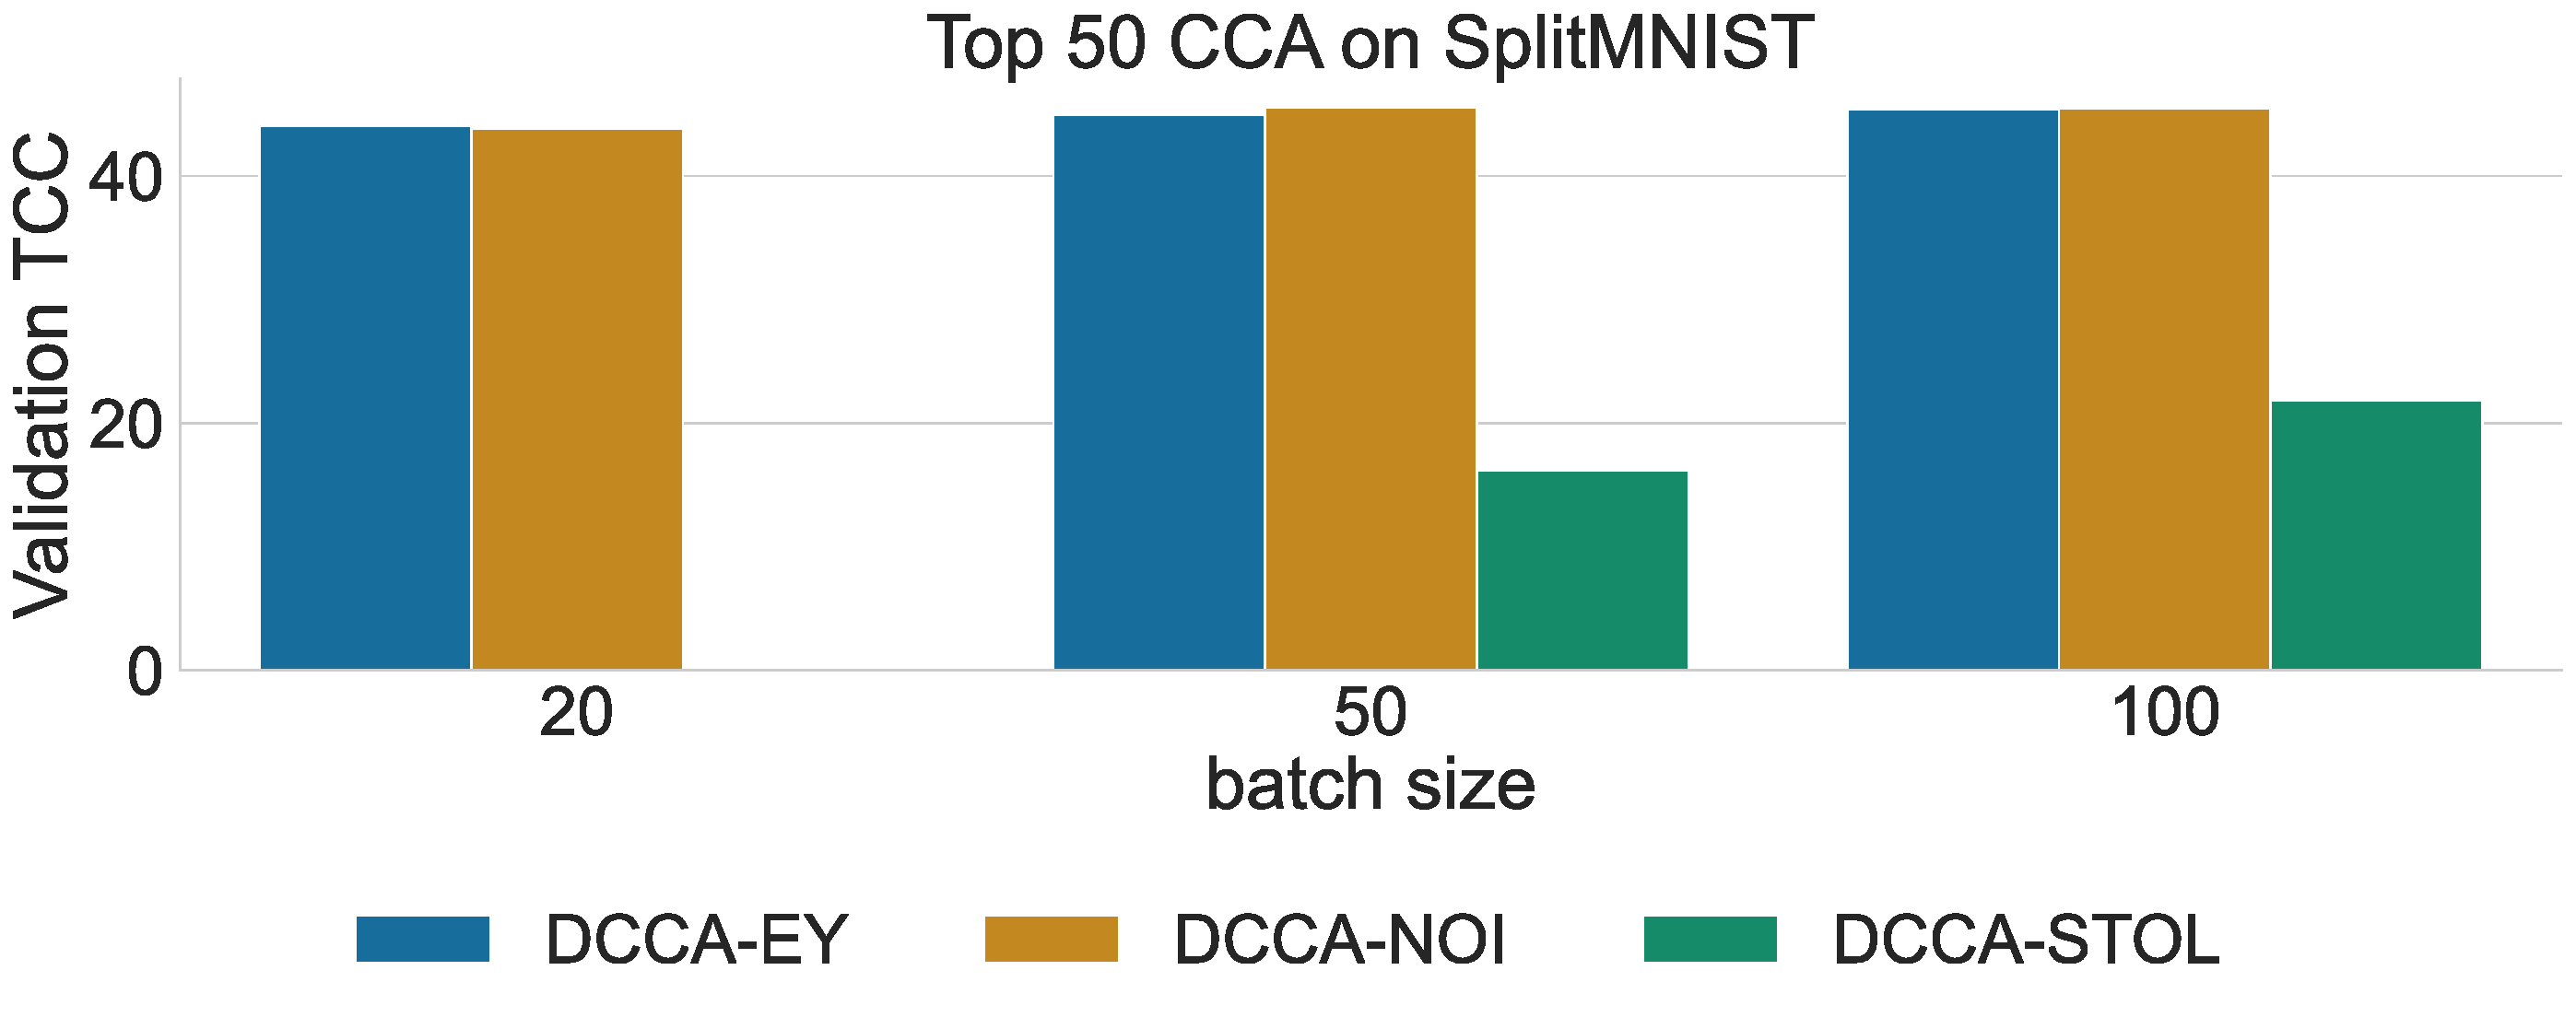
\includegraphics[width=0.8\textwidth]{figures/DCCA/SplitMNIST_models_different_batch_sizes}
    \caption{Deep CCA on SplitMNIST: Comparison of methods across varying batch sizes.}
    \label{fig:corr_mnist}
\end{figure}

\begin{figure}
    \centering
    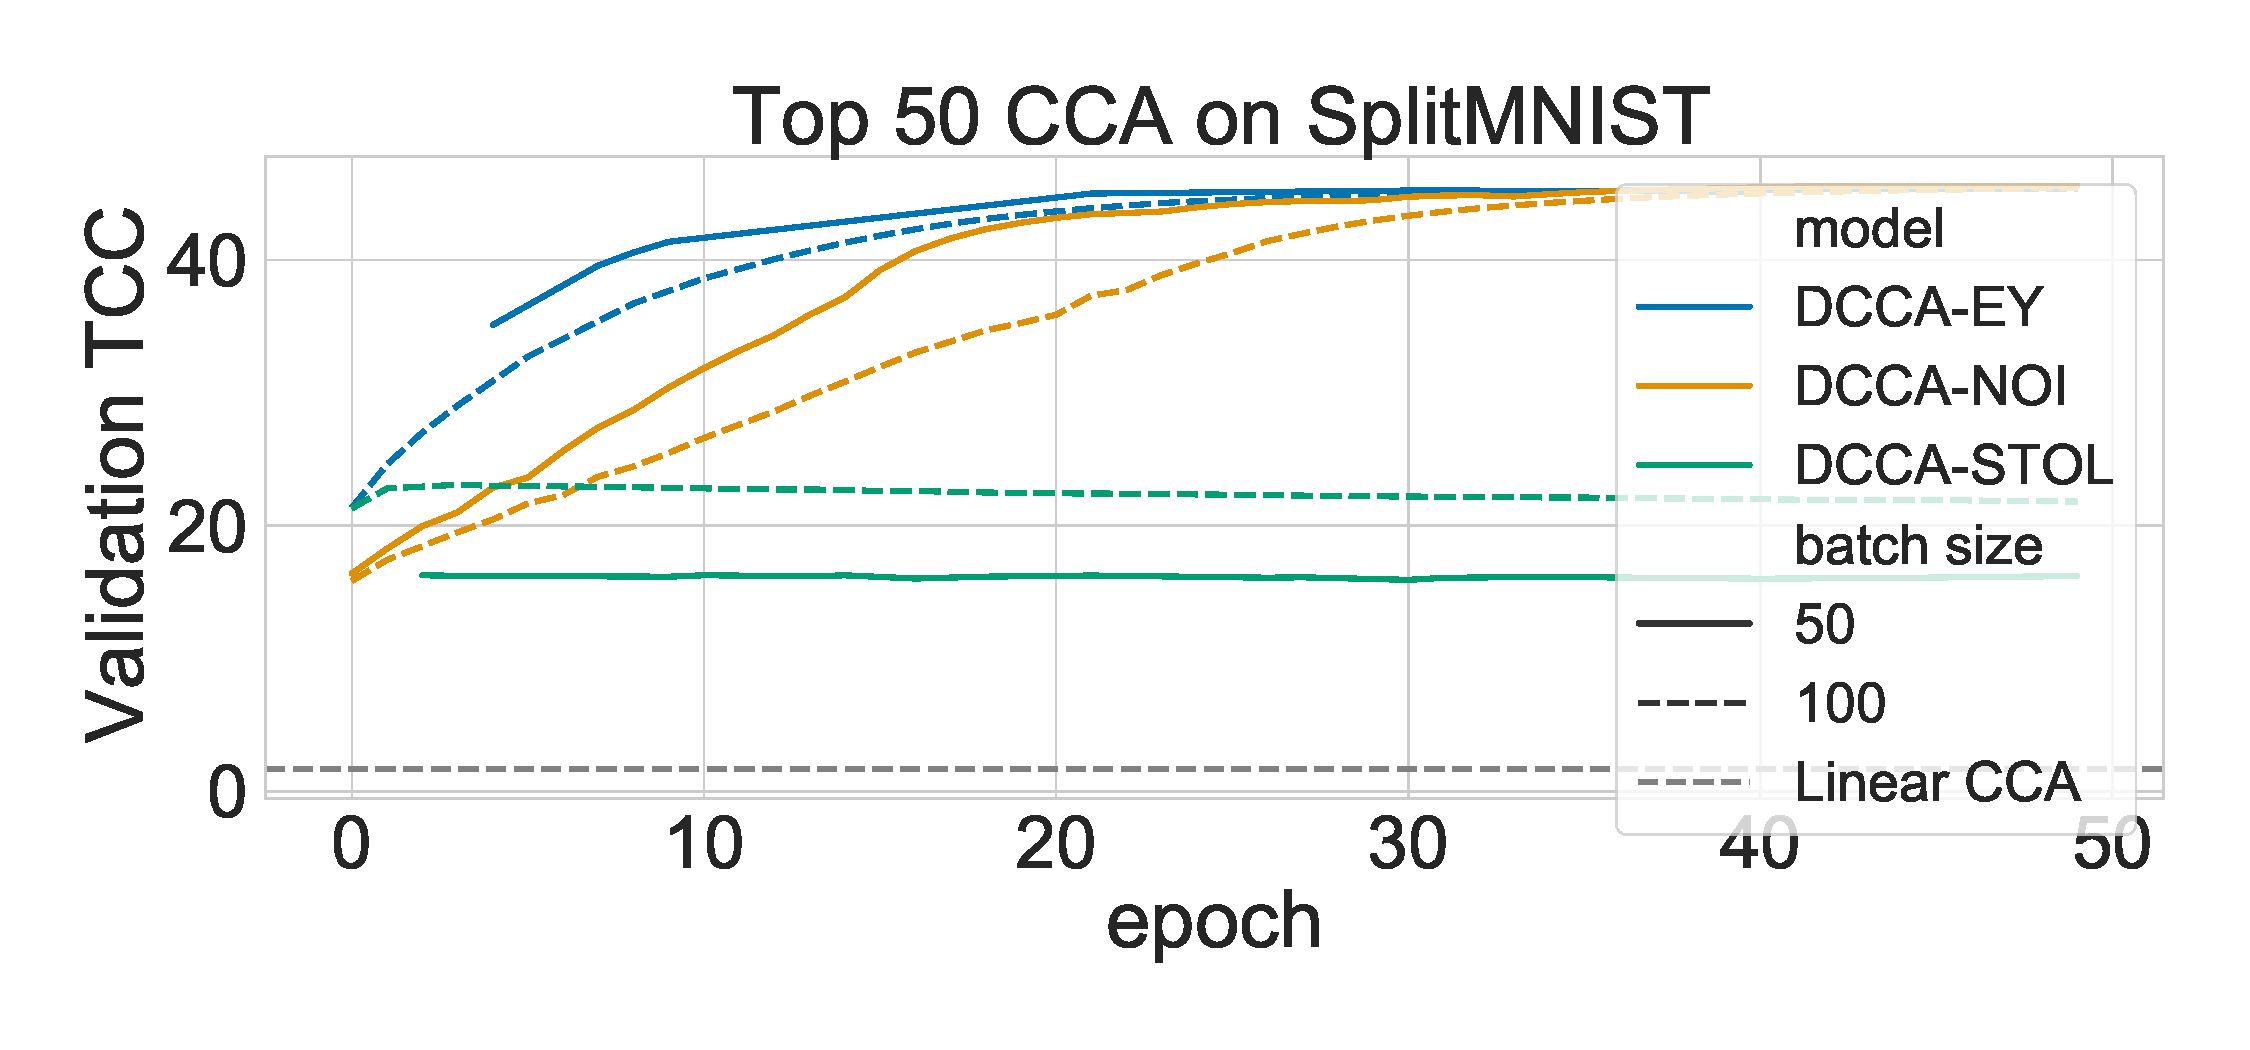
\includegraphics[width=0.8\textwidth]{figures/DCCA/SplitMNIST_allbatchsizes_pcc}
    \caption{Deep CCA on SplitMNIST: Learning progress over 50 epochs.}
    \label{fig:lr_mnist}
\end{figure}

\begin{figure}
    \centering
    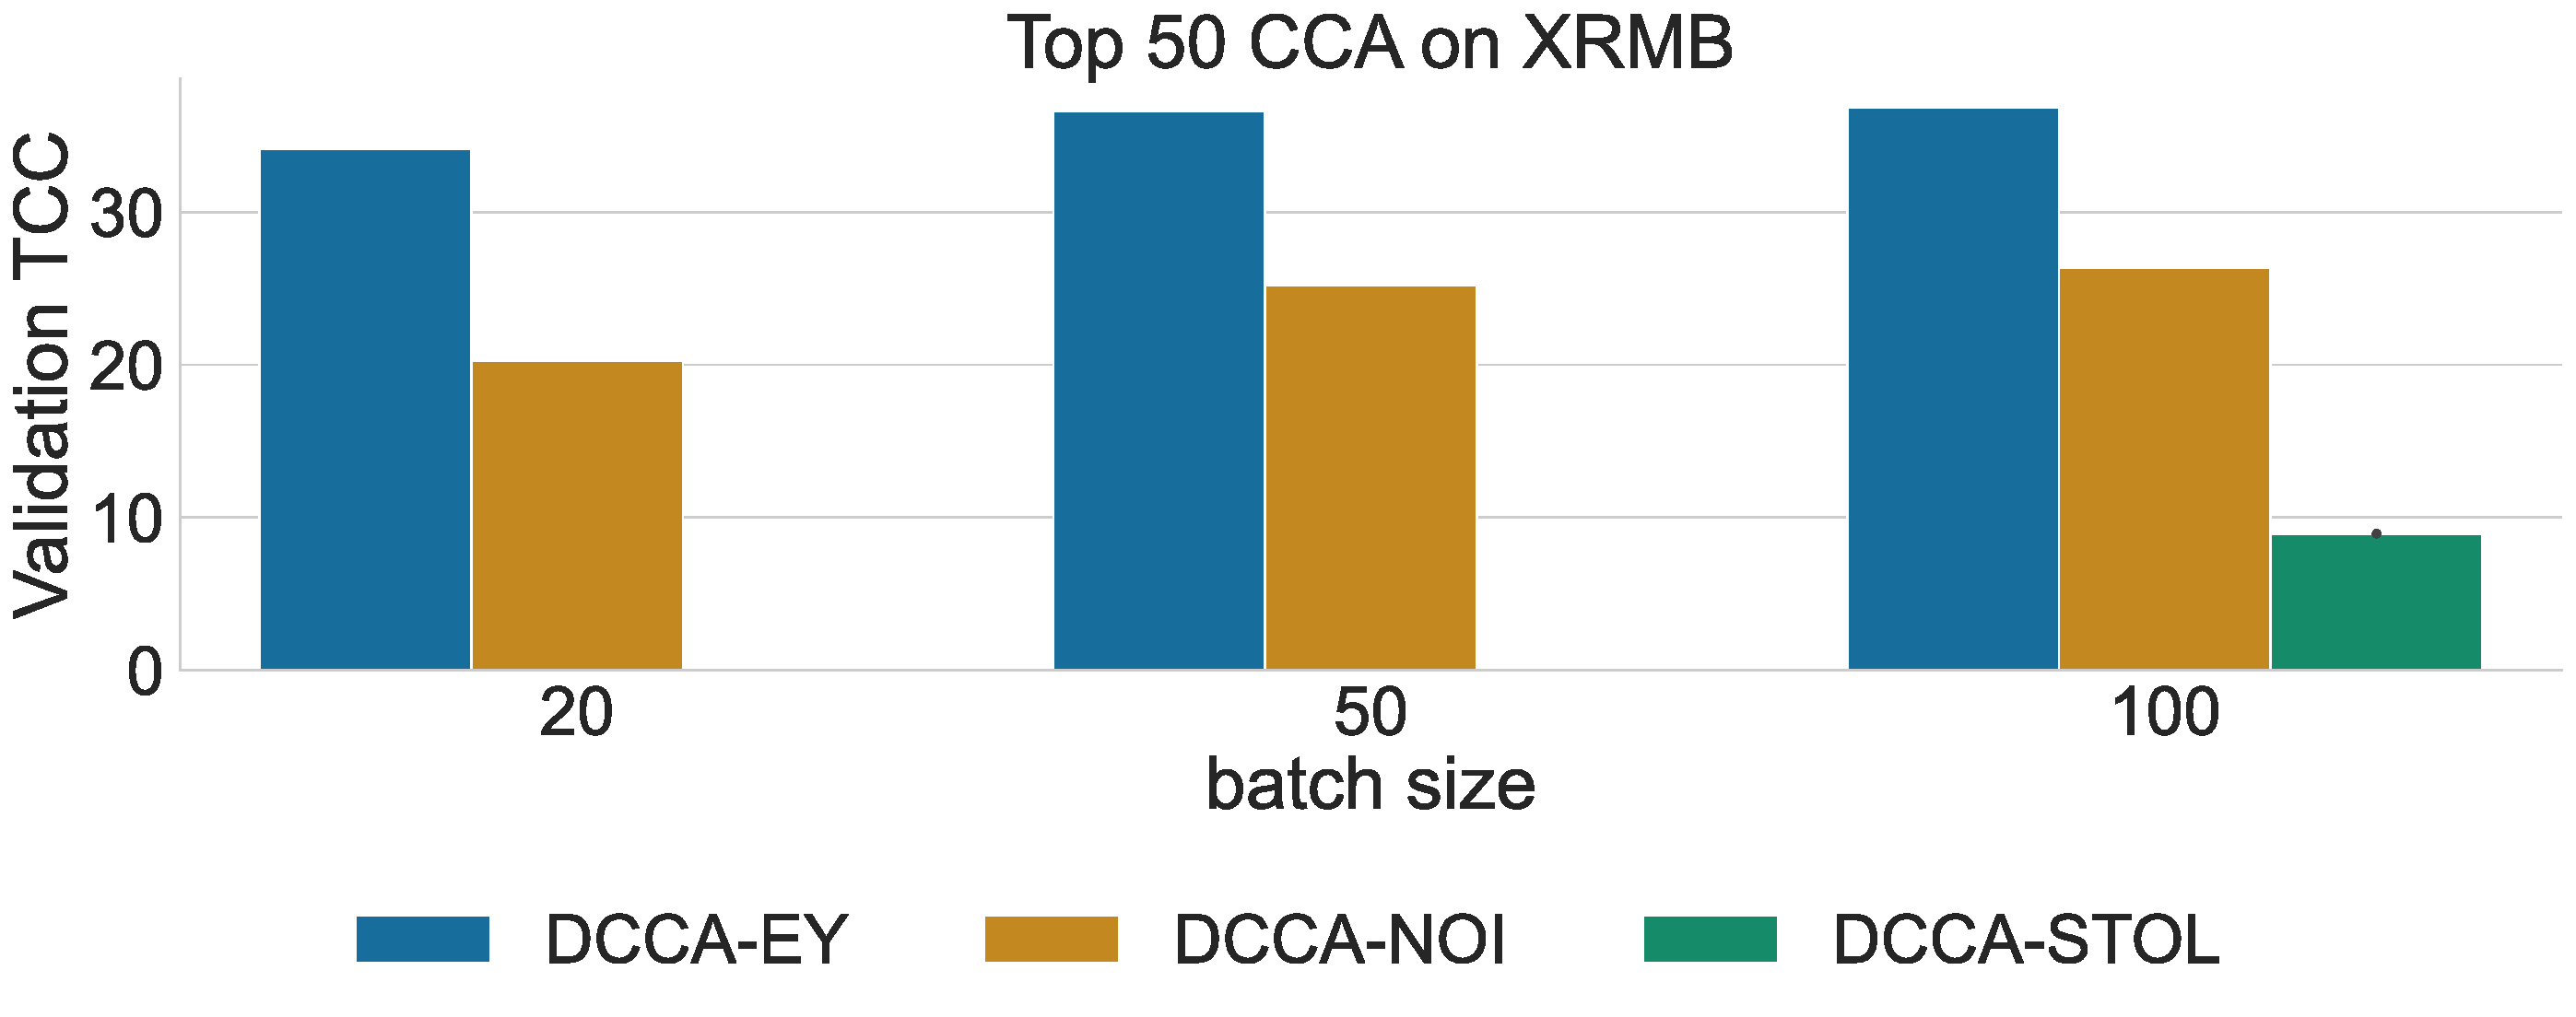
\includegraphics[width=0.8\textwidth]{figures/DCCA/XRMB_models_different_batch_sizes}
    \caption{Deep CCA on XRMB: Comparison of methods across varying batch sizes.}
    \label{fig:corr_xrmb}
\end{figure}

\begin{figure}
    \centering
    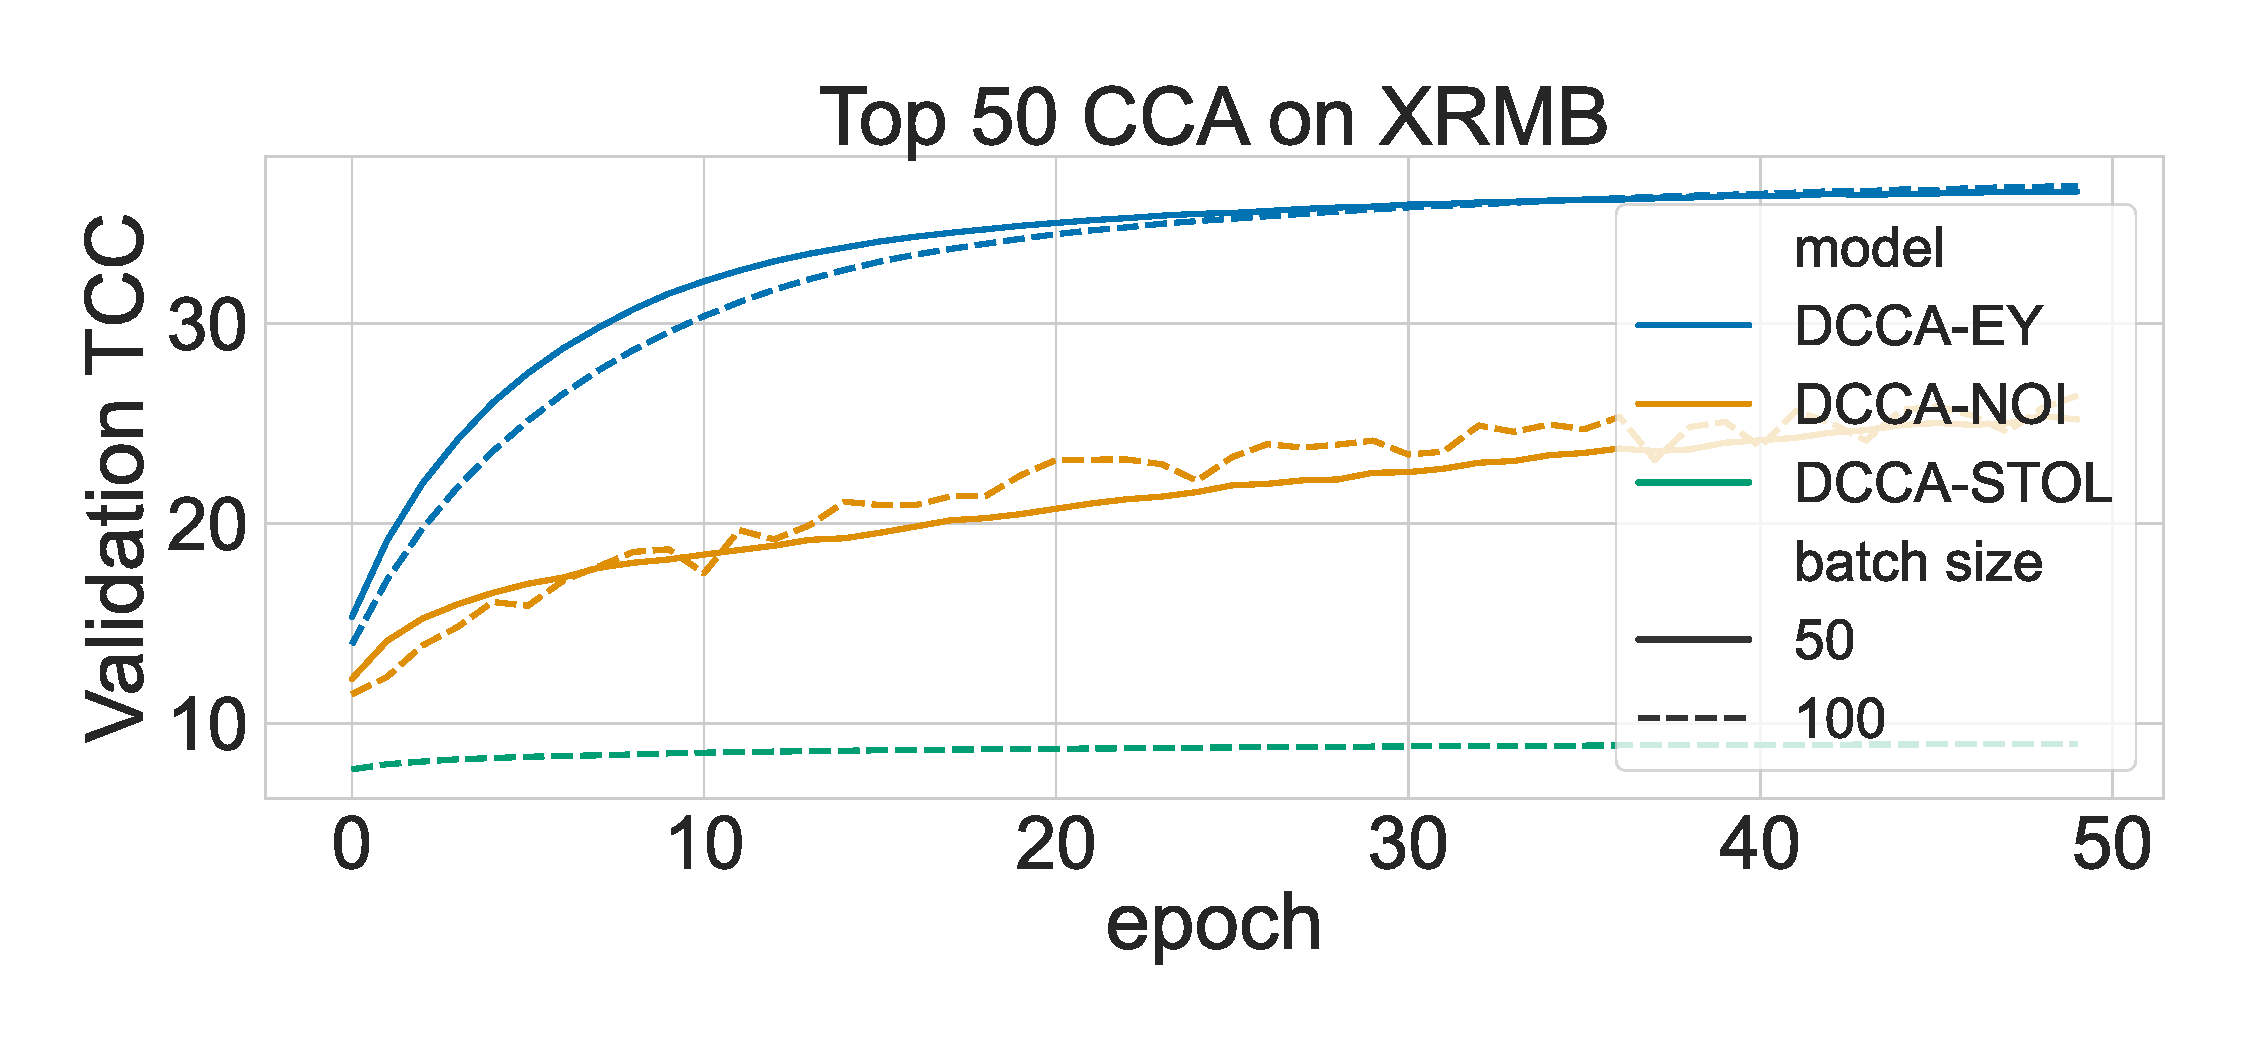
\includegraphics[width=0.8\textwidth]{figures/DCCA/XRMB_allbatchsizes_pcc}
    \caption{Deep CCA on XRMB: Learning progress over 50 epochs.}
    \label{fig:lr_xrmb}
\end{figure}

\subsection{Deep Multiview CCA: Robustness Across Different Batch Sizes}

In this experiment, we evaluate the performance and adaptability of our DCCA-EY method in a multiview context, comparing it against established multiview DCCA methods including Deep MCCA and Deep GCCA. Our primary goal is to assess how these methods perform across various batch sizes, with a particular focus on their ability to capture correlations between multiple views.

\subsubsection{Dataset: mfeat}

For this experiment, we utilize the mfeat dataset \citep{misc_multiple_features_72}, which provides an ideal testbed for multiview learning methods. This dataset consists of 2,000 handwritten numeral patterns, each represented by six distinct feature sets. These feature sets include Fourier coefficients, profile correlations, Karhunen-Love coefficients, pixel averages in 2x3 windows, Zernike moments, and morphological features.

The mfeat dataset is particularly valuable for our study due to its diverse feature types, which challenge the algorithms' ability to find correlations across heterogeneous data representations. This diversity allows us to assess the robustness and flexibility of our DCCA-EY method in dealing with varied data characteristics, a crucial aspect in real-world multiview learning scenarios.

\subsubsection{Experimental Setup}

Our experimental design aims to comprehensively evaluate the performance of various multiview Deep CCA methods across a range of batch sizes, with a particular focus on small batch scenarios. We hypothesize that our method will demonstrate superior performance across all batch sizes, but with a marked advantage in smaller batch conditions where existing methods are expected to struggle.

The core of our experiment involves training each Deep CCA variant to learn a shared representation space of 50 dimensions (K = 50). To ensure a thorough assessment of each method's convergence properties and final performance, we extend the training process over 100 epochs. This duration allows us to observe both the initial learning dynamics and the long-term stability of the learned representations.

A key aspect of our experimental design is the variation in batch sizes. We explore a wide spectrum, ranging from very small batches of 5 samples to larger batches of 200 samples. Specifically, we test batch sizes of 5, 10, 20, 50, 100, and 200. This range enables us to closely examine how each method's performance scales with increasing batch size, with particular attention to the challenging small-batch regime.

To ensure a fair comparison and to optimize each method's performance, we conduct a comprehensive hyperparameter search. The key hyperparameters and their ranges are summarized in Table \ref{tab:hyperparameters}.

\begin{table}[h!]
    \centering
    \caption{Hyperparameter ranges for Deep CCA methods}
    \label{tab:hyperparameters}
    \begin{tabular}{|l|l|}
        \hline
        Parameter                   & Values                    \\
        \hline
        Representation Dimensionality & 50                        \\
        Training Epochs             & 100                       \\
        Batch Sizes                 & 5, 10, 20, 50, 100, 200   \\
        Learning Rates              & 0.01, 0.001, 0.0001, 0.00001 \\
        \hline
    \end{tabular}
\end{table}

By systematically varying these parameters, particularly the batch size, we aim to provide a nuanced understanding of each method's strengths and limitations. Our analysis will focus on how performance metrics evolve across different batch sizes, with special attention to the small-batch scenarios where we anticipate our method to show significant advantages.

This experimental setup allows us to rigorously test our hypothesis that our proposed Deep CCA variant offers superior performance across a range of operational conditions, with a particular emphasis on its robustness in challenging small-batch scenarios. Through this comprehensive evaluation, we seek to demonstrate the practical advantages of our approach in real-world applications where small batch processing is often necessary due to computational or data streaming constraints.

\subsubsection{Evaluation Metric}

To effectively compare the performance of different methods in this multiview setting, we introduce a novel metric: the Total Multiview Correlation Captured (TMCC). This metric extends the concept of Total Correlation Captured to accommodate multiple views. The TMCC is defined as:

\[
    \text{TMCC} = \sum_{k=1}^{K} \frac{1}{I(I-1)} \sum_{\substack{i,j \leq I \\ i \neq j}} \text{corr}(Z_k^{(i)}, Z_k^{(j)}),
\]

where \( Z_k^{(i)} \) represents the \( k \)-th dimension of the \( i \)-th view's representation, and $I$ is the total number of views. This metric quantifies the average correlation across all pairs of views for each dimension of the learned representations. A higher TMCC indicates better capture of inter-view correlations, reflecting the method's effectiveness in learning a shared multiview representation.

\subsubsection{Objectives}

Our experiment is designed with several key objectives. First, we aim to evaluate DCCA-EY's performance in capturing multiview correlations, comparing it directly with Deep MCCA and Deep GCCA. Second, we seek to assess the robustness of these methods across a wide range of batch sizes, from very small (5) to relatively large (200).

\subsubsection{Observations}
Figure~\ref{fig:dmcca_corr} illustrates the comparison of DCCA-EY with Deep GCCA and Deep MCCA across different mini-batch sizes, using the validation TMCC metric.
DCCA-EY consistently outperforms both Deep GCCA and Deep MCCA, showcasing its superior ability to capture validation TMCC. Notably, Deep MCCA encounters issues when the batch size is smaller than $K=50$, likely due to singular empirical covariances.
Deep GCCA, while not breaking down, significantly underperforms with smaller batch sizes, highlighting limitations in scalability and efficiency for large-scale data applications.

In Figure~\ref{fig:dmcca_lr}, we observe the learning curves for batch sizes 50 and 100. Both Deep MCCA and Deep GCCA demonstrate rapid initial learning of significant correlations but reach a plateau relatively quickly. In contrast, DCCA-EY exhibits a consistent improvement over time and notably outperforms the other methods by the end of the training period. This behavior underscores the enhanced learning capability and efficiency of DCCA-EY, especially in the context of large-scale, high-dimensional data.

\begin{figure}
    \centering
    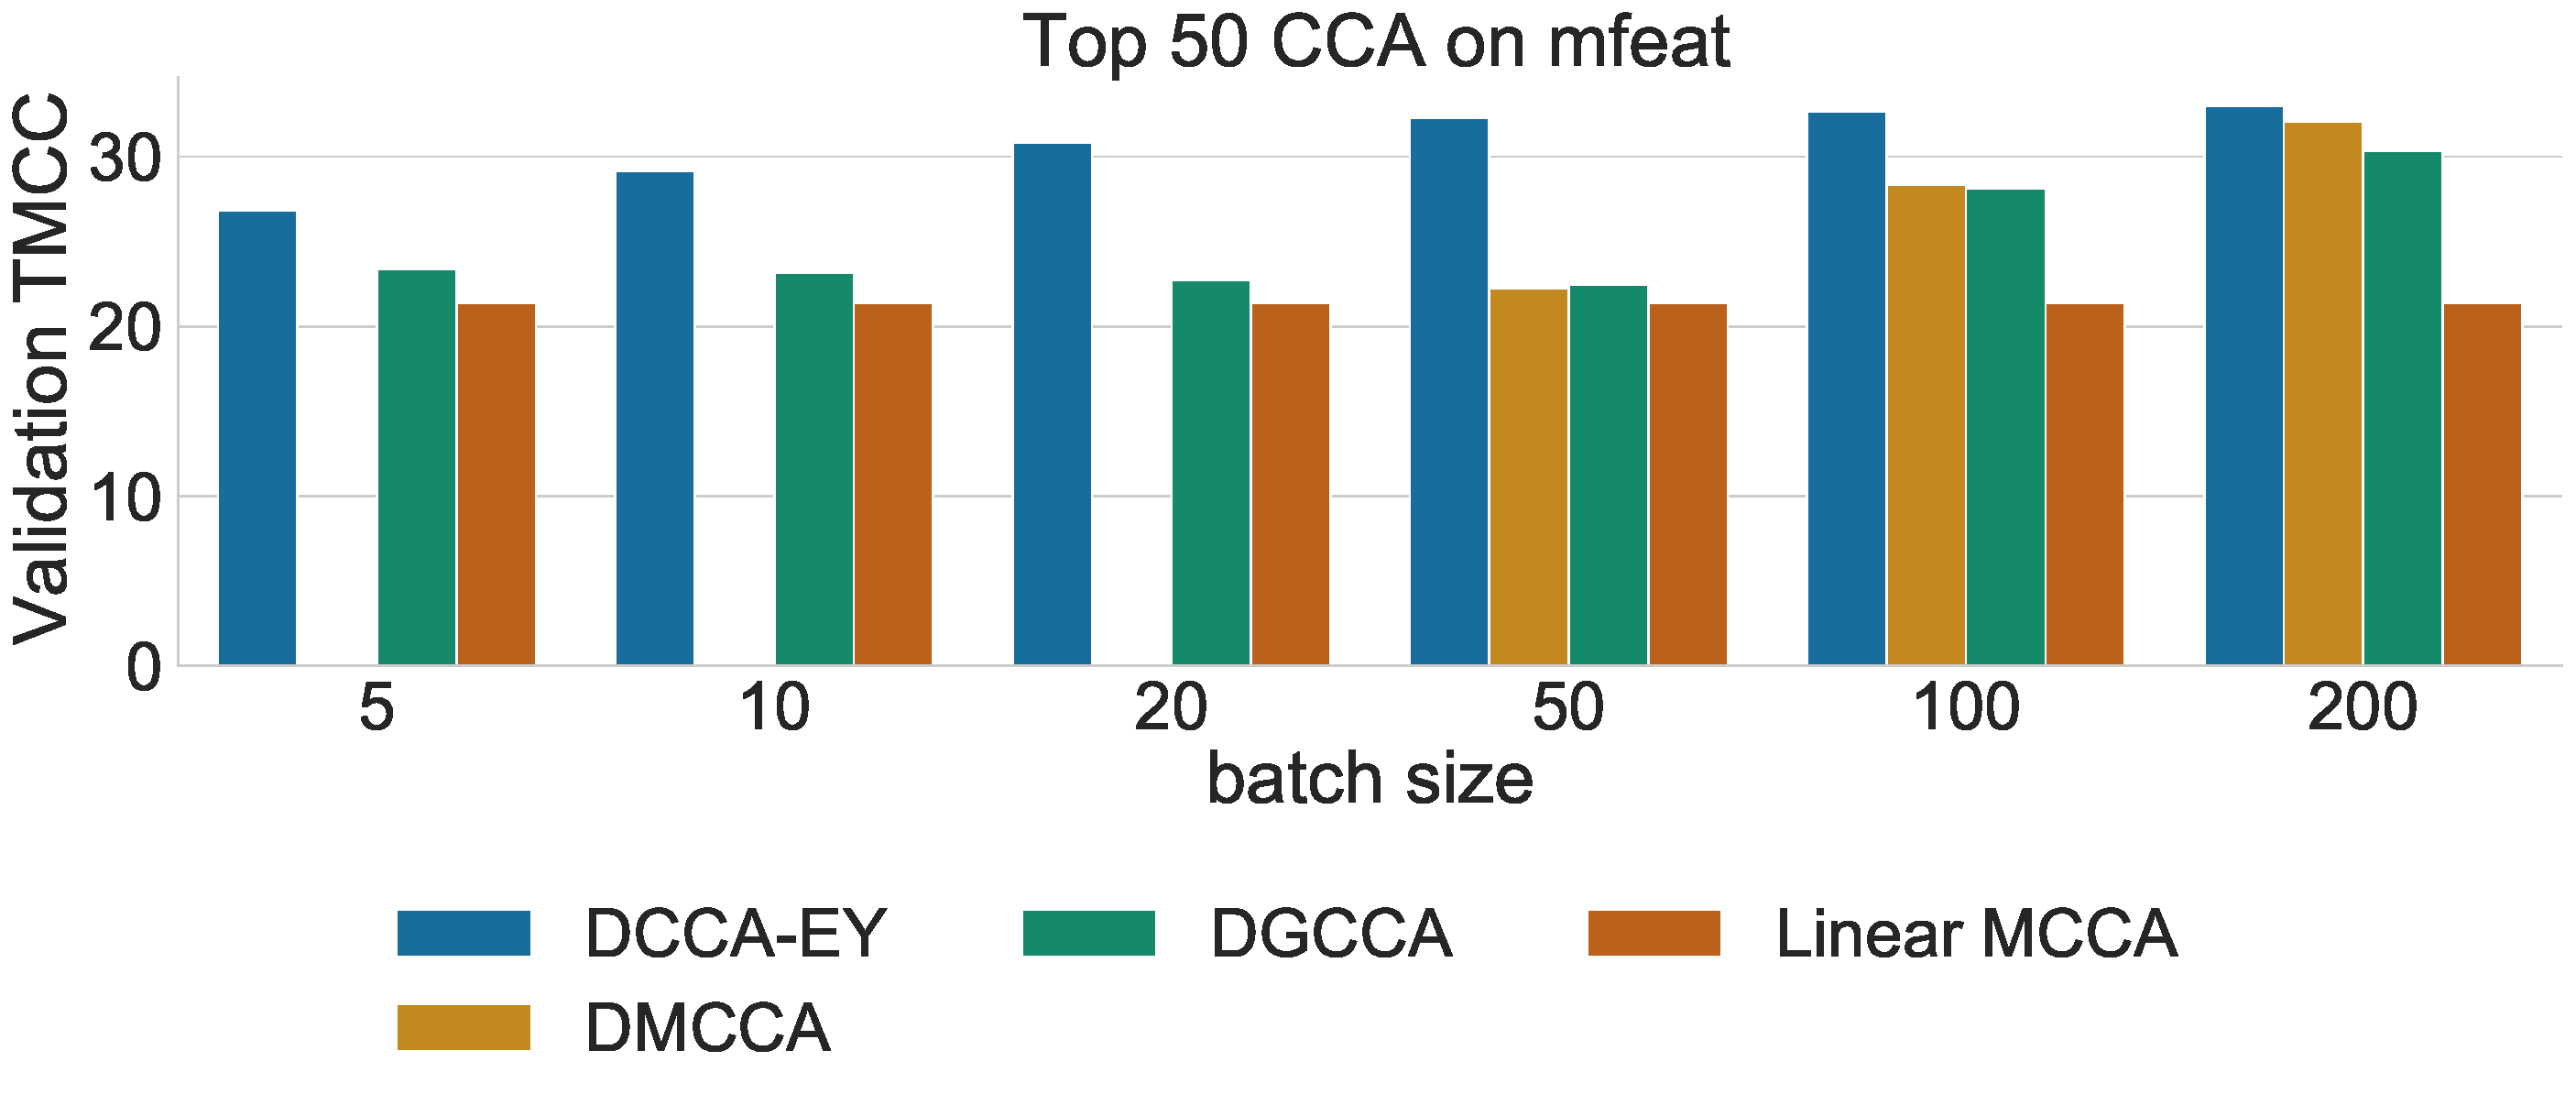
\includegraphics[width=0.8\textwidth]{figures/DMCCA/mfeat_models_different_batch_sizes}
    \caption{Deep Multi-view CCA on mfeat: Comparison across various mini-batch sizes using the Validation TMCC metric.}\label{fig:dmcca_corr}
\end{figure}

\begin{figure}
    \centering
    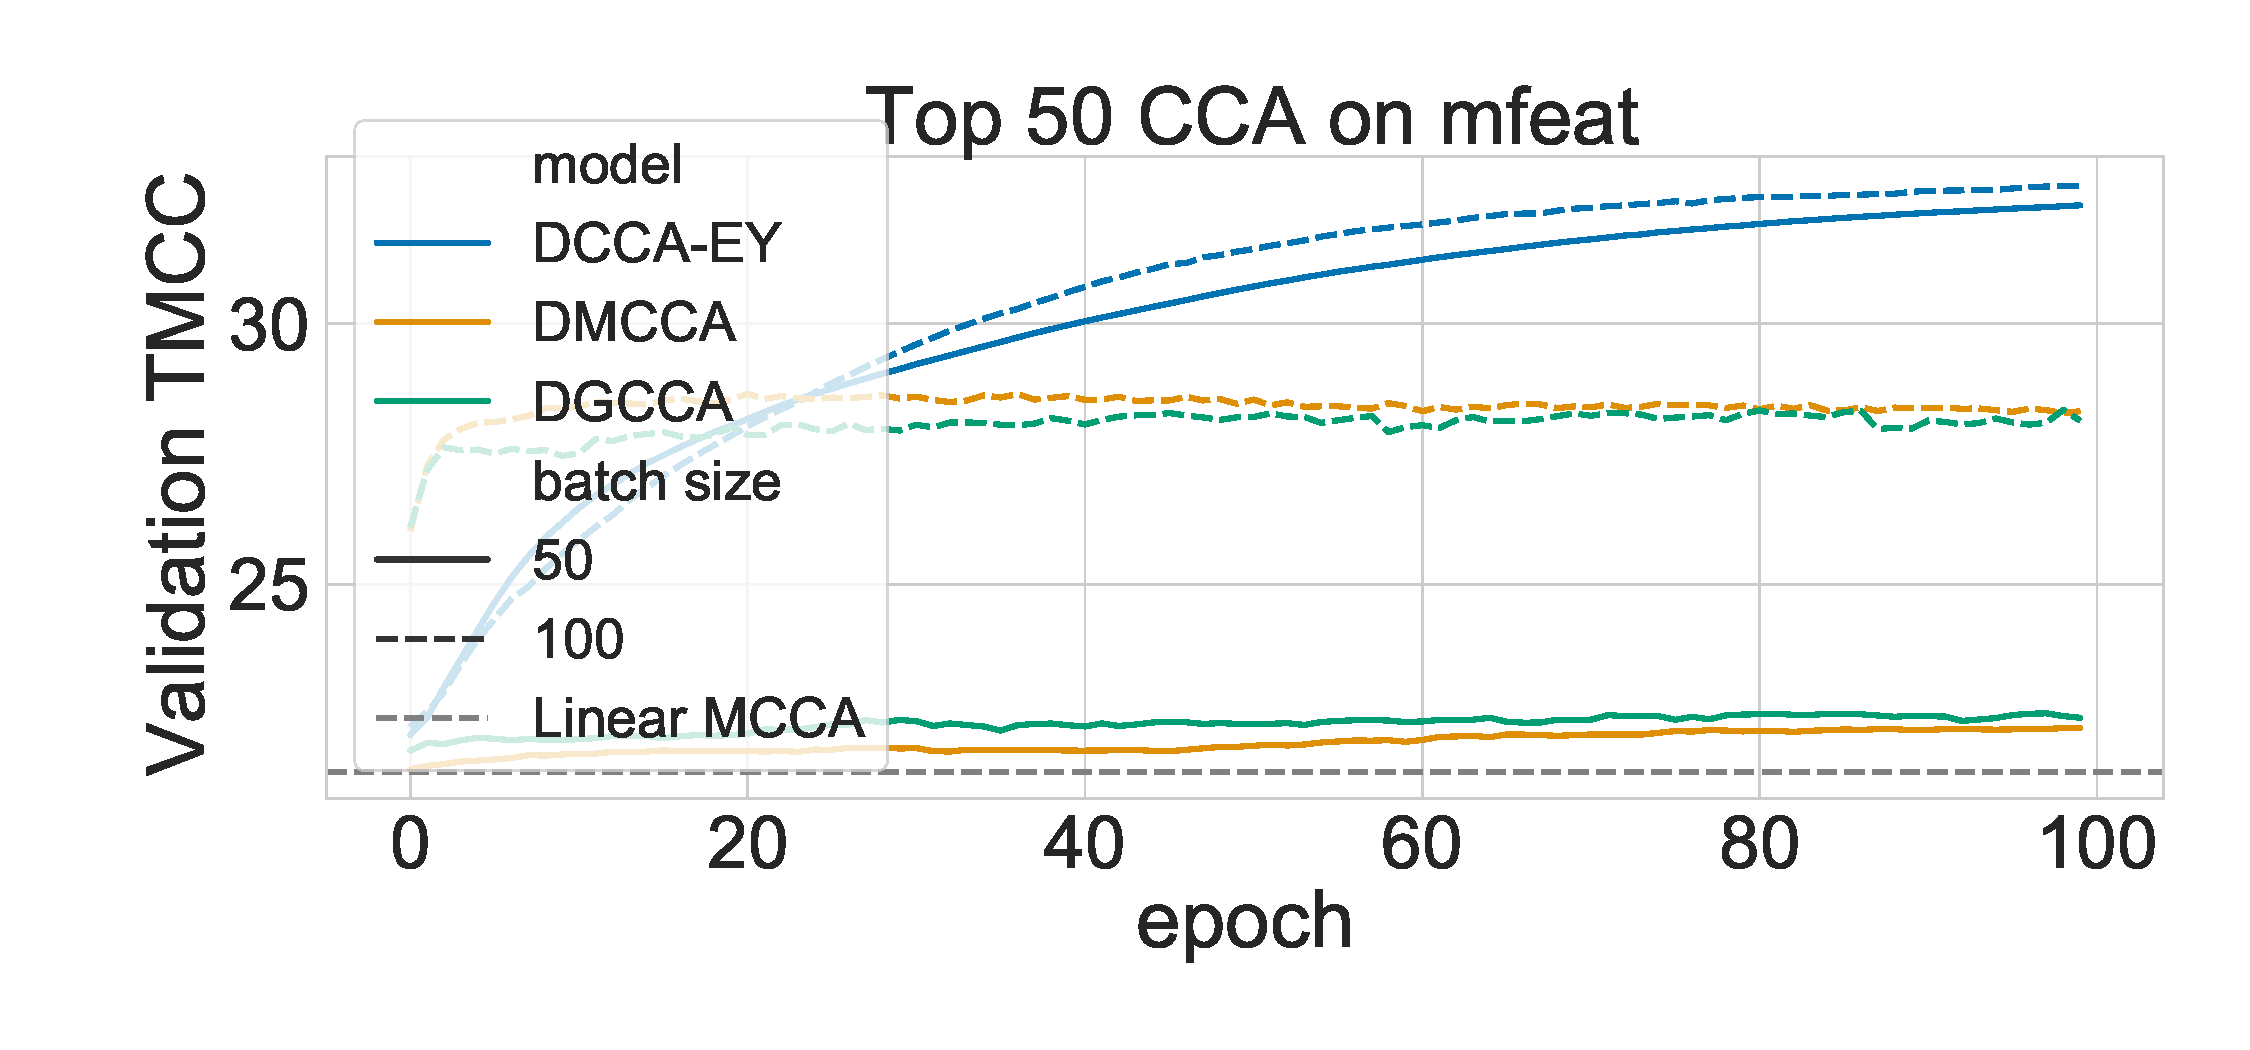
\includegraphics[width=0.8\textwidth]{figures/DMCCA/mfeat_allbatchsizes_pcc}
    \caption{Deep Multi-view CCA on mfeat: Learning progress over 100 epochs for batch sizes 50 and 100.}\label{fig:dmcca_lr}
\end{figure}

\subsection{Self-Supervised Learning with SSL-EY}

To evaluate the effectiveness of our proposed SSL-EY method in self-supervised learning tasks, we conduct a comprehensive benchmark comparison against two established baselines: Barlow Twins and VICReg. This experiment aims to assess SSL-EY's performance in learning meaningful representations from unlabeled data.

\subsubsection{Datasets}

We evaluate our method on two widely-used benchmark datasets: CIFAR-10 and CIFAR-100. Both datasets consist of 60,000 32x32 color images, divided into 50,000 training images and 10,000 test images.

CIFAR-10 contains images from 10 classes, with 6,000 images per class. This dataset provides a balanced representation of basic object categories, offering a good starting point for evaluating self-supervised learning methods.

CIFAR-100, on the other hand, presents a more challenging scenario with 100 classes and only 600 images per class. This increased number of classes and reduced per-class sample size tests the methods' ability to learn discriminative features in a more fine-grained classification setting.

These datasets provide a diverse range of image complexities and class structures, allowing for a comprehensive evaluation of SSL-EY's performance across different scenarios. The contrast between CIFAR-10 and CIFAR-100 enables us to assess how well each method scales with increasing task complexity.

\subsubsection{Experimental Setup}
We follow a standardized experimental design as outlined in \citet{tong2023emp}, utilizing the sololearn library \citep{da2022solo}. This library provides optimized setups specifically tailored for VICReg and Barlow Twins, ensuring a fair comparison.

Key aspects of the setup include:
\begin{itemize}
    \item \textbf{Encoder}: ResNet-18 architecture
    \item \textbf{Projector}: Bi-layer network
    \item \textbf{Training Duration}: 1,000 epochs
    \item \textbf{Batch Size}: 256 images
    \item \textbf{SSL-EY Hyperparameters}: Adopted from Barlow Twins optimization
\end{itemize}

For SSL-EY, we intentionally use the hyperparameters that were optimized for Barlow Twins. This choice aims to demonstrate SSL-EY's robustness and adaptability rather than seeking to outperform existing methods through extensive tuning.

\subsubsection{Evaluation Methodology}
To assess the quality of the learned representations, we employ a linear probe approach:

\begin{enumerate}
    \item Train the self-supervised models on the unlabeled training data.
    \item Fix the encoder weights and train a linear classifier on top of the learned representations using the labeled training data.
    \item Evaluate the classifier's performance on the validation set using two metrics:
        \begin{itemize}
            \item \textbf{Top-1 Accuracy}: Percentage of samples where the highest probability prediction matches the true label.
            \item \textbf{Top-5 Accuracy}: Percentage of samples where the true label is among the top 5 highest probability predictions.
        \end{itemize}
\end{enumerate}

This approach allows us to gauge how well the self-supervised methods capture meaningful and discriminative features from the unlabeled data.
It is important to note that in our figures, we actually present log accuracy rather than raw accuracy. Log accuracy provides a more revealing representation of performance differences, especially when comparing models with high accuracy scores. This is because small improvements in raw accuracy at higher levels can represent significant performance gains, which are more clearly visible on a logarithmic scale.

By comparing SSL-EY against Barlow Twins and VICReg under these controlled conditions, we aim to provide insights into its effectiveness as a self-supervised learning algorithm, particularly its ability to learn robust and transferable representations across different datasets and task complexities.

\subsubsection{Observations} As Table \ref{tab:selfsup} demonstrates, SSL-EY rivals Barlow Twins and VICReg, despite employing general hyperparameters as opposed to the latter's specifically optimized ones.

\begin{table}[H]
    \centering
    \caption{Comparison of SSL method performance on CIFAR-10 and CIFAR-100 datasets.}
    \resizebox{\textwidth}{!}{%
    \begin{tabular}{|l|c|c|c|c|}
        \hline
        Method          & CIFAR-10 Top-1 & CIFAR-10 Top-5 & CIFAR-100 Top-1 & CIFAR-100 Top-5 \\
        \hline
        Barlow Twins    & \textbf{92.1}  & 99.73          & \textbf{71.38}  & \textbf{92.32}  \\
        \hline
        VICReg          & 91.68          & 99.66          & 68.56           & 90.76           \\
        \hline
        \textbf{SSL-EY} & 91.43          & \textbf{99.75} & 67.52           & 90.17           \\
        \hline
    \end{tabular}
    }
    \label{tab:selfsup}
\end{table}

\subsubsection{Model Convergence}
Figure \ref{fig:ssl_learning_curve} illustrates the learning curve analysis for both CIFAR-10 and CIFAR-100 datasets.

\begin{figure}[H]
    \begin{subfigure}[b]{0.48\textwidth}
        \centering
        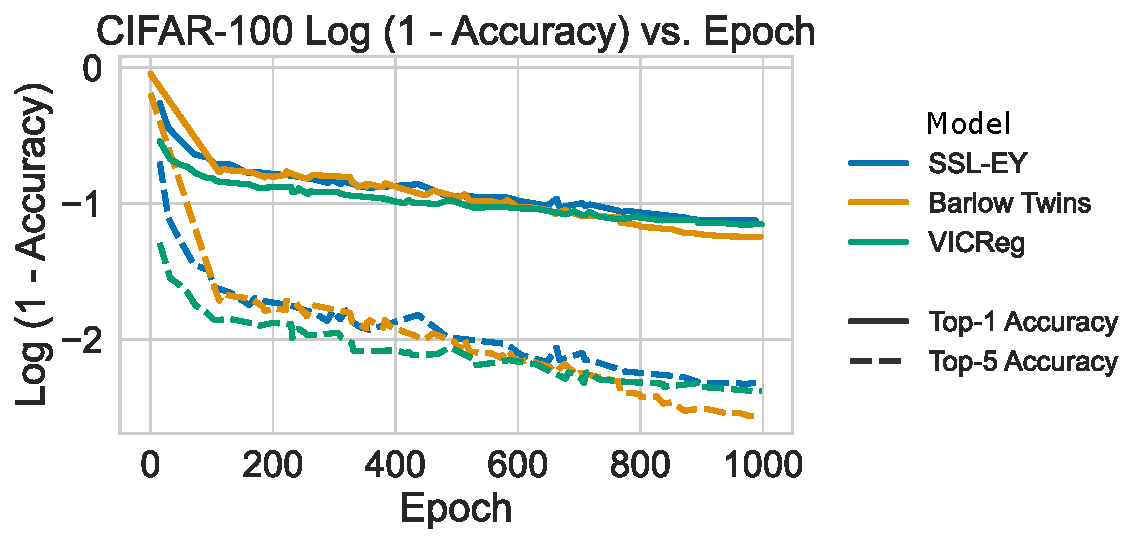
\includegraphics[width=\textwidth]{figures/SSL/cifar100_learning_curve_log_error}
        \caption{CIFAR-100}
        \label{fig:ssl_learning_curve_cifar100}
    \end{subfigure}
    \hfill
    \begin{subfigure}[b]{0.48\textwidth}
        \centering
        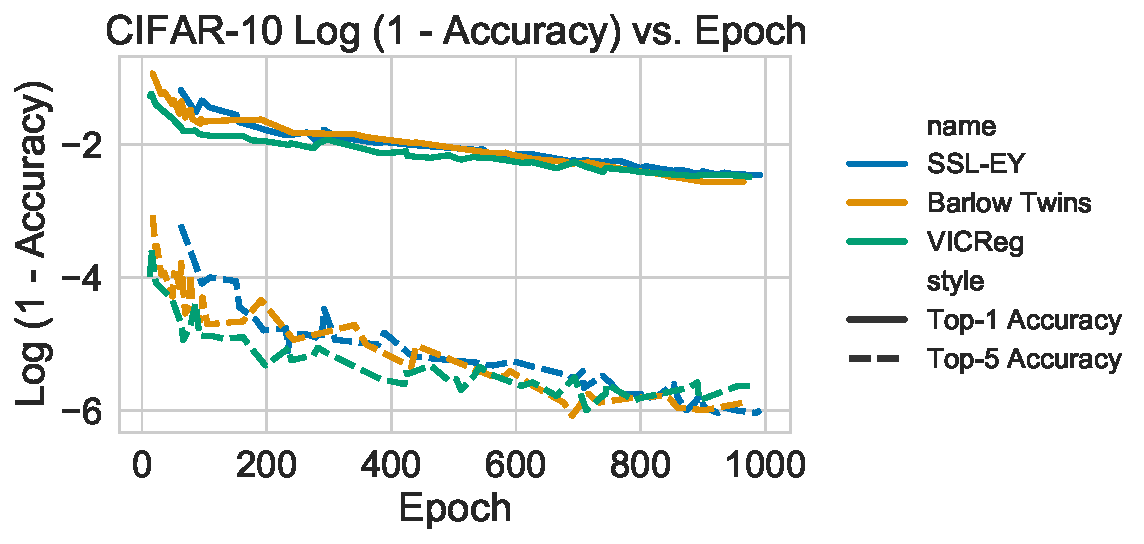
\includegraphics[width=\textwidth]{figures/SSL/cifar10_learning_curve_log_error}
        \caption{CIFAR-10}
        \label{fig:ssl_learning_curve_cifar10}
    \end{subfigure}
    \caption{Learning curves for SSL-EY, Barlow Twins, and VICReg, depicting 1,000-epoch performance.}
    \label{fig:ssl_learning_curve}
\end{figure}

The learning curves in Figure \ref{fig:ssl_learning_curve} reveal a crucial insight: all compared SSL methods converge at remarkably slow rates, with hundreds of epochs required for significant performance improvements. Even after 1,000 epochs, the models continue to learn. This observation highlights a significant advantage of SSL-EY: its ability to achieve competitive performance without extensive hyperparameter tuning.

The performance variations at 1,000 epochs, as shown in Table \ref{tab:selfsup}, primarily stem from optimization noise, with convergence speeds being comparable among methods. This slow convergence underscores the importance of SSL-EY's robustness to hyperparameter choices, as it can achieve competitive results without the need for time-consuming fine-tuning.

\subsubsection{Projector Size Variation and No-Projector Performance}
We hypothesized that SSL-EY's architecture might exhibit robustness to projector size, potentially allowing for efficient performance even with smaller projectors or without one entirely. To investigate this, we conducted experiments varying the projector dimensions across SSL-EY, Barlow Twins, and VICReg, including a scenario with no projector. Figure \ref{fig:ssl_projector_dim} presents our findings on both CIFAR-100 and CIFAR-10 datasets.

\begin{figure}[H]
    \begin{subfigure}[b]{0.48\textwidth}
        \centering
        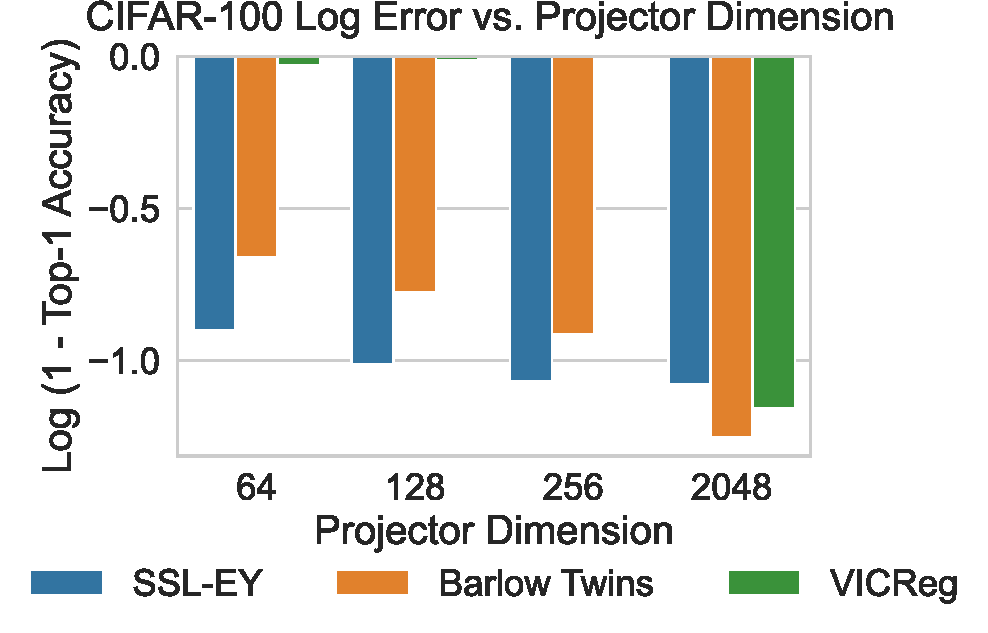
\includegraphics[width=\textwidth]{figures/SSL/cifar100_proj_dim_log_error}
        \caption{CIFAR-100}
        \label{fig:ssl_projector_dimensions_100}
    \end{subfigure}
    \hfill
    \begin{subfigure}[b]{0.48\textwidth}
        \centering
        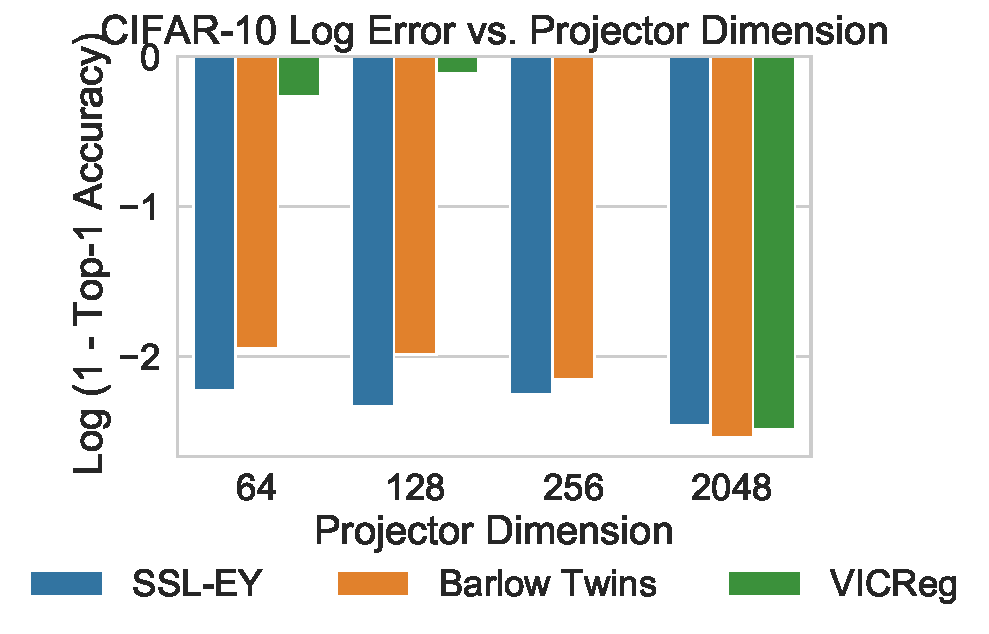
\includegraphics[width=\textwidth]{figures/SSL/cifar10_proj_dim_log_error}
        \caption{CIFAR-10}
        \label{fig:ssl_projector_dimensions_10}
    \end{subfigure}
    \caption{Impact of projector size on SSL-EY, Barlow Twins, and VICReg performance for CIFAR-100 and CIFAR-10 datasets. The y-axis shows log error (inversely related to log accuracy), while the x-axis represents projector dimensions.}
    \label{fig:ssl_projector_dim}
\end{figure}

Figure \ref{fig:ssl_projector_dim} reveals that SSL-EY demonstrates remarkable stability across various projector sizes, maintaining high performance even as dimensions are reduced. In contrast, Barlow Twins and VICReg show more significant performance degradation with smaller projector sizes, particularly on the more complex CIFAR-100 dataset.

To further investigate the impact of removing the projector entirely, we conducted additional experiments applying the linear probe directly to the encoder outputs. Table \ref{tab:noprojector} presents these results alongside the projector-based performance for all three methods.

\begin{table}[H]
    \centering
    \caption{Comparison of SSL method performance with and without projector on CIFAR-10 and CIFAR-100 datasets.}
    \resizebox{\textwidth}{!}{%
    \begin{tabular}{|l|c|c|c|c|c|}
        \hline
        Method          & Projector & CIFAR-10 Top-1 & CIFAR-10 Top-5 & CIFAR-100 Top-1 & CIFAR-100 Top-5 \\
        \hline
        Barlow Twins    & Yes       & \textbf{92.1}  & 99.73          & \textbf{71.38}  & \textbf{92.32}  \\
        Barlow Twins    & No        & 89.99          & 99.21          & 63.51           & 86.99           \\
        \hline
        VICReg          & Yes       & 91.68          & 99.66          & 68.56           & 90.76           \\
        VICReg          & No        & \textbf{90.99} & 99.46          & 63.82           & 86.39           \\
        \hline
        \textbf{SSL-EY} & Yes       & 91.43          & \textbf{99.75} & 67.52           & 90.17           \\
        \textbf{SSL-EY} & No        & 90.98          & 99.69          & \textbf{65.21}  & \textbf{88.09}  \\
        \hline
    \end{tabular}
    }
    \label{tab:noprojector}
\end{table}

The results in Table \ref{tab:noprojector} provide several key insights:

\begin{itemize}
    \item Both Barlow Twins and VICReg show a notable drop in performance when the projector is removed, particularly on the more complex CIFAR-100 dataset.
    \item SSL-EY demonstrates remarkable resilience, maintaining competitive performance even without a projector. This is especially evident on CIFAR-100, where SSL-EY's no-projector performance surpasses that of Barlow Twins and VICReg.
    \item On CIFAR-10, all methods show less dramatic changes when the projector is removed, likely due to the dataset's lower complexity.
\end{itemize}

These findings strongly support our initial hypothesis, highlighting SSL-EY's unique capacity to learn robust and efficient representations with minimal architectural overhead. The method's consistent performance across datasets of varying complexity and its resilience to projector removal underscore its versatility and potential for broad applicability in self-supervised learning tasks.

Despite the similarities in the underlying motivations across all three methods, our results suggest that a projector may not be a mandatory component for correlation-based models, at least in the context of our proposed method. By achieving competitive results with reduced architectural requirements, SSL-EY not only offers computational advantages but also suggests a more fundamental efficiency in its approach to representation learning.

\subsubsection{$\LEY$ as an Informative Metric}
A significant challenge in self-supervised learning (SSL) is tuning models to ensure their learned representations are robust and generalizable across various potential downstream tasks. Traditionally, SSL methods are often tuned using classification accuracy as a proxy metric. However, this approach risks overfitting the model to the specific classification task, potentially compromising its versatility for other applications. This practice contradicts the fundamental goal of SSL: to create representations that are adaptable to a wide range of unforeseen challenges.

To address this issue, we propose that our EY loss ($\LEY$) could serve as a more appropriate surrogate metric for tuning and monitoring SSL models. By using $\LEY$ instead of classification accuracy, we aim to maintain the model's generality while still providing a meaningful measure of representational quality. This approach aligns more closely with the core principles of SSL, potentially leading to more versatile and robust learned representations.

To explore this possibility, we investigated the relationship between EY loss and classification accuracy. Our findings, presented in Figure \ref{fig:ssl_ey_vs_acc}, offer compelling evidence for the potential of $\LEY$ as an informative metric in SSL training.

\begin{figure}[H]
    \begin{subfigure}[b]{0.48\textwidth}
        \centering
        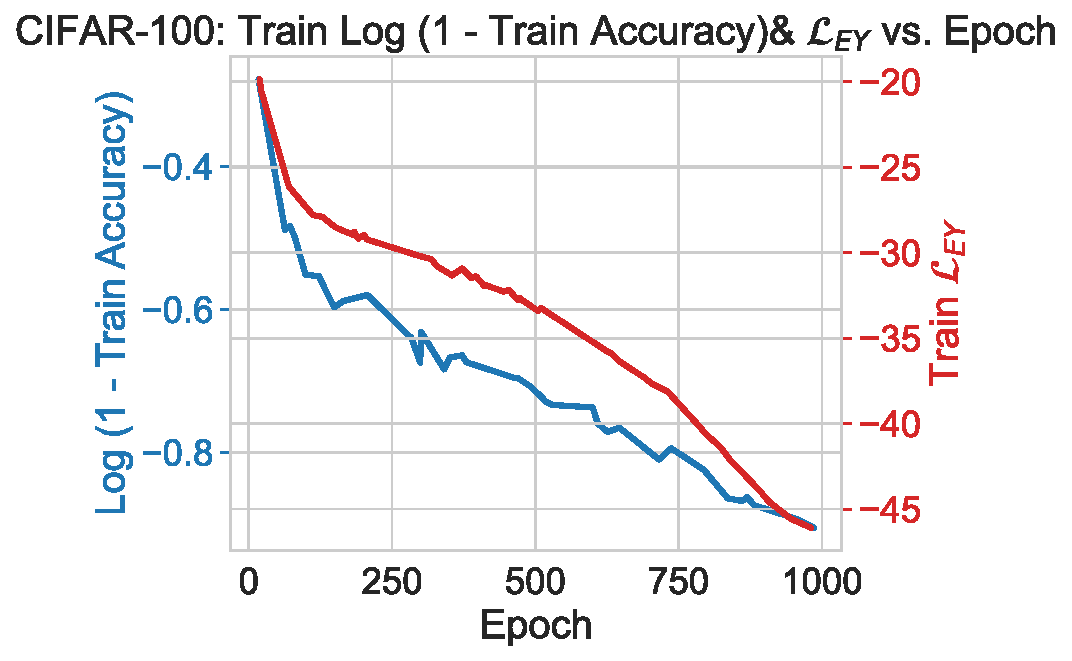
\includegraphics[width=\textwidth]{figures/SSL/cifar100_corr_vs_acc_log_error}
        \caption{CIFAR-100}
        \label{fig:ssl_learning_curve_cifar100_vs_corr}
    \end{subfigure}
    \hfill
    \begin{subfigure}[b]{0.48\textwidth}
        \centering
        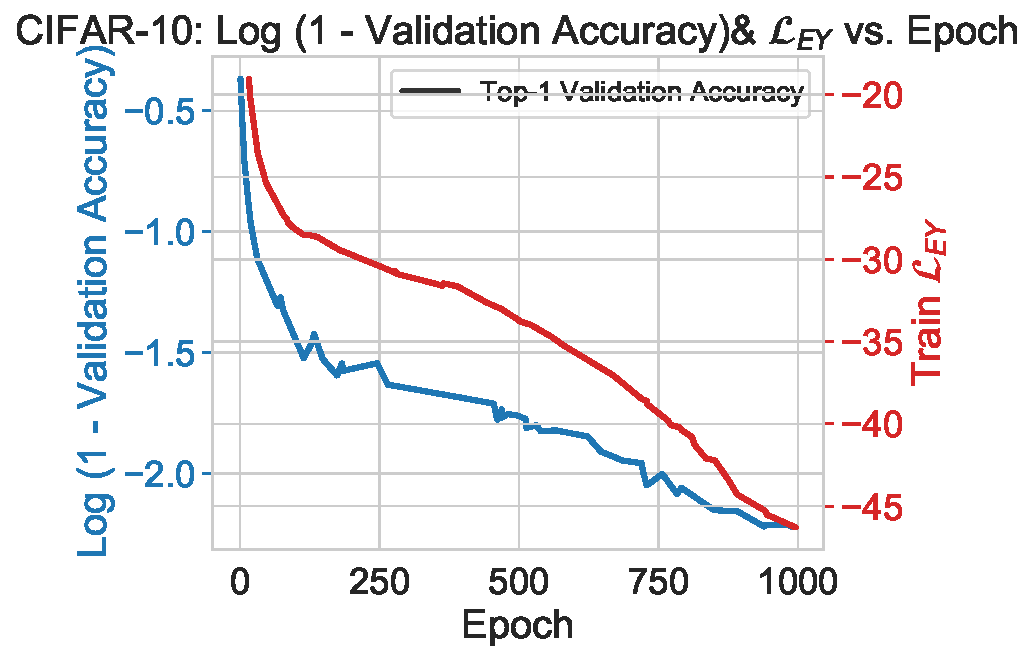
\includegraphics[width=\textwidth]{figures/SSL/cifar10_corr_vs_acc_log_error}
        \caption{CIFAR-10}
        \label{fig:ssl_learning_curve_cifar10_vs_corr}
    \end{subfigure}
    \caption{Correlation between EY loss and classification accuracy for CIFAR-100 and CIFAR-10 datasets.}
    \label{fig:ssl_ey_vs_acc}
\end{figure}

The correlation between EY loss and classification accuracy, shown in Figure \ref{fig:ssl_ey_vs_acc}, offers two key insights:

\begin{enumerate}
    \item The strong relationship between EY loss and classification accuracy highlights the potential of maximizing canonical correlation as a pretext task in SSL.
    \item The sustained increase in correlation over 1,000 epochs suggests that even with reduced projector dimensionality, SSL-EY does not reach full capacity, indicating untapped potential in its representation capacity.
\end{enumerate}

The evolution of the correlation, measured by $\LEY$, suggests a new avenue for monitoring model training, potentially eliminating the need for a separate validation task. These results collectively demonstrate SSL-EY's robustness, efficiency, and potential for simplifying the self-supervised learning process across different dataset complexities.

This analysis not only supports the use of $\LEY$ as a valuable monitoring tool for SSL training but also highlights its potential to streamline the development process. By providing a metric that correlates strongly with downstream performance without being tied to a specific task, $\LEY$ could offer a more principled approach to model tuning in self-supervised learning contexts.

\section{Discussion and Limitations}

\subsection{Discussion}

This chapter introduces DCCA-EY and SSL-EY, novel approaches that address key limitations in Deep CCA and Self-Supervised Learning methods. These innovations offer significant advantages in terms of scalability, convergence speed, and robustness to hyperparameter tuning, making them valuable tools for practitioners in representation learning.

One of the most notable strengths of DCCA-EY is its superior performance across various mini-batch sizes, as evidenced by our experiments on the Split MNIST and XRMB datasets. This scalability is crucial for handling large-scale datasets and diverse computational environments, a common challenge in modern machine learning applications. Moreover, both DCCA-EY and SSL-EY demonstrate faster convergence compared to existing methods, a particularly valuable trait in SSL tasks where training often requires a large number of epochs.

The reduced sensitivity to hyperparameter choices shown by our methods is another significant advantage. In practical applications, where extensive tuning can be prohibitively time-consuming or computationally expensive, this robustness can greatly streamline the deployment process. SSL-EY's ability to maintain performance with reduced or absent projectors suggests more efficient representation learning, potentially leading to simpler architectures and reduced computational requirements.

Furthermore, the observed correlation between EY loss and classification accuracy in SSL-EY provides a novel way to monitor training progress without relying on labeled validation data. This insight opens up new possibilities for unsupervised learning scenarios and could lead to more efficient training protocols.

\subsection{Limitations}

However, despite these advancements, our work is not without limitations. While our experiments were comprehensive, they were limited to specific datasets (Split MNIST, XRMB, CIFAR-10, CIFAR-100). Future research should explore performance on a broader range of datasets, including those from different domains such as natural language processing and time series data. This would provide a more complete picture of the methods' generalizability and robustness across diverse data types.

Additionally, while we have demonstrated improved scalability, further research is needed to assess performance on very large models and extremely high-dimensional datasets, which are increasingly common in cutting-edge machine learning applications. A more in-depth theoretical analysis of why DCCA-EY and SSL-EY perform well, particularly in stochastic settings, could provide valuable insights and guide future improvements.

Although our methods show improved convergence, a detailed study of their computational requirements compared to existing methods would be beneficial, especially for resource-constrained environments. Exploring how DCCA-EY and SSL-EY can be combined with other advanced techniques in deep learning, such as attention mechanisms or adaptive learning rates, could potentially lead to even better performance.

While our methods improve performance, further work on enhancing the interpretability of the learned representations could increase their utility in domains where model explainability is crucial. Our experiments, while extensive, were limited to 1,000 epochs. Investigating the long-term stability and performance of our methods over even longer training periods could provide insights into their asymptotic behavior.

\section*{Conclusion}

In conclusion, DCCA-EY and SSL-EY represent significant advancements in Deep CCA and Self-Supervised Learning, offering improved scalability, faster convergence, and robustness to hyperparameter choices. These qualities make them valuable tools for researchers and practitioners working with complex, high-dimensional data. The strong performance of our methods, even without extensive tuning, suggests that they capture fundamental aspects of correlation and representation learning. This not only enhances their practical utility but also opens up new avenues for theoretical exploration in the fields of multiview learning and self-supervised learning.